
\documentclass[10pt,twocolumn]{article}
\usepackage[margin=0.75in,columnsep=0.25in]{geometry}
\usepackage{amsmath,amssymb,amsfonts}
\usepackage{booktabs}
\usepackage{longtable}
\usepackage{graphicx}
\usepackage{xcolor}
\usepackage{algorithm}
\usepackage{algpseudocode}
\usepackage[hidelinks]{hyperref}
\usepackage{natbib}

\renewcommand{\topfraction}{0.9}\renewcommand{\dbltopfraction}{0.9}\renewcommand{\bottomfraction}{0.8}
\renewcommand{\textfraction}{0.07}\renewcommand{\floatpagefraction}{0.75}\renewcommand{\dblfloatpagefraction}{0.75}
\setcounter{topnumber}{4}\setcounter{dbltopnumber}{4}\setcounter{totalnumber}{6}
\raggedbottom
\makeatletter\setlength{\@fptop}{0pt}\setlength{\@dblfptop}{0pt}\makeatother
\newcommand{\sign}{\operatorname{sign}}
\newcommand{\R}{\mathbb{R}}

\title{Training Ternary Language Models Without Master Weights}
\author{Ozgur Guzeldereli \\ University College London}
\date{29 October 2026}

\begin{document}
\maketitle

\begin{abstract}
Ternary (1.58-bit) language models are cheap to run, but published methods train them with a full-precision copy of every weight (master-weight) and Adam's two moments which is 12 bytes of training state per weight. Ablating master-weight training one part at a
time shows what a ternary network needs from it. It needs an integrator of normalised gradient evidence with a memory of about a
thousand steps, which decides when a weight changes, and an immediate change when the integral crosses a
threshold boundary. It needs neither a full-rank first moment nor a per-weight second moment. From these parts we
build a master-free rule, \emph{two-timescale threshold flips} (TTF). The
Adam-normalised gradient, with a Adafactor-style factored second moment, feeds a leaky accumulator kept at low rank, and a ternary
weight moves one level when its accumulated evidence crosses a threshold, spending the threshold. TTF's gap to master
weights is a smooth function of the size of its state and closes at 0.57--0.70 numbers of state per weight from 110M to
2.9B parameters. At 110M, TTF leads master given the same auxiliary float parameters by 0.044 nats at 300M tokens, and at
1.3B and 2.9B it is level. The lead does not come from the float parameters. Without them TTF still leads master that
has them, and with a ternary embedding on both TTF and master, with only scales and norm gains in float, its lead grows to 0.12. A 15M ternary model trained
from scratch with TTF stays 0.11 nats behind its full-precision twin on FineWeb-Edu from one to five times compute-optimal training.
With half a byte of state per weight, a 23B-parameter model trains on one 16 GB GPU.
\end{abstract}

\section{Introduction}

Ternary weights $\{-1,0,1\}$ take 1.58 bits each instead of 16, about a tenth of the memory, and replace
most multiplications by additions \citep{ma2024era}. Ternary models trained from scratch with enough tokens approach
full-precision models of the same size \citep{ma2024era,kaushal2025spectra}. Training them is expensive in memory.
Published recipes keep a full-precision latent copy of each weight (the \emph{master weights}), quantise the latent-weight in the
forward pass, passes the gradient straight through the quantiser \citep{bengio2013estimating,courbariaux2015binaryconnect},
and runs Adam on the latent. The optimizer state is then three fp32 numbers per weight (latent and two moments, 12 bytes),
sixty times the 0.2 bytes a packed trit occupies. The memory wall that ternary weights remove at inference is still there
in training. It is there again when an existing full-precision model is quantised to ternary weights and its accuracy
recovered by training, and the recovery needs about 16 bytes per weight, several times the memory of the model it starts
from.

This paper asks \emph{what the master copy does for a ternary network}, and whether a rule that keeps only that part
can train without it.

\paragraph{Approach.} We ablate master-weight training one part at a time (Section~\ref{sec:ablation}). The latent
of a ternary weight is a position inside a cell of the quantiser, and the trit changes when the position crosses a cell
boundary. Master training needs a slow integrator (about a thousand steps of memory) that decides when a weight changes,
and needs the change to happen the moment the boundary is crossed. It needs neither a full-rank first moment nor a
per-weight second moment. We then build a rule from exactly these parts without a latent copy: TTF
(Section~\ref{sec:method}). The integrator's state is stored at low rank. Written at full rank, TTF is close to a master
latent with a leak, a snap to the new cell and a factored, momentum-free Adam (Section~\ref{sec:fullrank}). The memory saving,
and the method's claim, is the low-rank storage of the not-yet-spent evidence while every spent move lands in the
full-rank trits.

\paragraph{What we find.} TTF trains ternary language models from scratch as well as or better than master weights
given the same auxiliary float parameters: 0.044 nats ahead at 110M parameters and 300M tokens, 0.056 ahead at 600M
tokens, 0.032 ahead at 340M, and level at 1.3B and 2.9B with the state sizes we could afford there. Its result depends
smoothly on one quantity, the size of its state. At every size we trained, from 110M to 2.9B parameters, it reaches master
at 0.57--0.70 stored numbers per weight, about one byte at the 12-bit precision the accumulator tolerates, against twelve
bytes for master. Below that, each halving of the state costs a fixed amount, which gets smaller as model size grows. We trace both
facts to measured properties of the gradient. A step spreads its energy evenly over octaves of directions, because the
layers' inputs do, while the part of the gradient that persists over a thousand steps needs a rank that grows almost in
proportion to the width. Because the trits move in discrete steps, TTF responds to the learning-rate schedule
differently from master. A decaying step can freeze it, which an annealed leak prevents, and late training becomes a
phase of rare moves that are each worth more than master's. The ternary network keeps pace with longer training. A
15M model trained from scratch with TTF stays 0.11 nats behind full precision trained on the same tokens on FineWeb-Edu, at one, two
and five times compute-optimal (Section~\ref{sec:depth15}). The same update also converts pretrained models to ternary
weights and keeps training them, which is the subject of a companion paper.

\paragraph{Organisation.} Section~\ref{sec:setup} defines the ternary layers, the master-weight reference and the
evaluation. Section~\ref{sec:ablation} ablates master training and Section~\ref{sec:method} builds TTF from what it needs.
Sections~\ref{sec:baselines}--\ref{sec:results} compare the two methods from 110M to 2.9B parameters,
Section~\ref{sec:rank} measures and explains the role of the state's size, Section~\ref{sec:dynamics} the dynamics under
the learning-rate schedule, Section~\ref{sec:organise} how ternary networks trained from scratch differ from full
precision, Section~\ref{sec:floatfree} models without float parameters, Section~\ref{sec:memory}
memory and speed (the conversion of pretrained models is the companion paper's subject), and Section~\ref{sec:discussion}
what the change from a memory to a compute bound means, including for misuse. Every mechanism we built or tested
is indexed with its result in Appendix~\ref{app:index}. We also publish the code that reproduced all of the results below.

\paragraph{Contributions.}
\begin{enumerate}
\item An ablation of master-weight training for ternary networks that shows what the master copy provides, a long
  integrator and immediate threshold crossing (Section~\ref{sec:ablation}).
\item TTF, a master-free update whose only per-weight state is the trit. Its optimizer state is a factored second moment
  and a rank-$r$ leaky accumulator, $r(N+K)+N+K$ numbers per $N\times K$ layer (Section~\ref{sec:method}).
\item The loss of TTF as a function of the size of its state, at four model sizes. The trade-off is log-linear, the same
  at 1.3B and 2.9B, and reaches master at about 0.7 numbers per weight (Section~\ref{sec:rank}). We add per-layer
  adaptive rank and a rank schedule (Section~\ref{sec:adaptive}).
\item Comparisons at 110M, 340M, 1.3B and 2.9B parameters on Wikipedia and FineWeb-Edu against master weights with
  exactly the same auxiliary float parameters, a momentum-free one-float master, and a low-rank Adam straight-through
  baseline (Sections~\ref{sec:baselines}--\ref{sec:results}).
\item An account of how threshold-flip training responds to the learning-rate schedule (Section~\ref{sec:dynamics}): a
  freeze under a decaying step and its fix, and a decomposition of late-training progress into the number of moves and
  the value of each move, for TTF and master.
\item A float-free variant in which the embedding and output head are ternary too (Section~\ref{sec:floatfree}), and a
  measured memory and speed budget, including a micro-batch update that never forms a dense gradient
  (Section~\ref{sec:memory}).
\item The ternary gap under longer training. A 15M model trained from scratch with TTF stays a constant 0.11 nats
  behind its full-precision twin from one to five times compute-optimal training (Section~\ref{sec:depth15}).
\item A comparison of ternary networks trained from scratch with full precision at 110M: no massive activations,
  higher effective rank, separate but equally good basins, and sharper minima in continuous directions but not along
  the lattice (Section~\ref{sec:organise}).
\end{enumerate}

\section{Background and setup}\label{sec:setup}

\subsection{Ternary layers}
A ternary linear layer holds trits $T\in\{-1,0,1\}^{N\times K}$, packed five per byte (1.6 bits per weight). Its forward
pass is
\begin{equation}
  y = r\odot\big(\beta\,T\,(c\odot x) + P\,Q^\top(c\odot x)\big), \qquad \beta = \frac{1}{\sqrt{K\rho_T}},
\end{equation}
with $\rho_T$ the share of nonzero trits (a variance-preserving scale computed from the trits, not stored), learned row
and column scales $r\in\R^N$, $c\in\R^K$, and a rank-16 additive float term $PQ^\top$. Attention has a learned per-head
temperature. Activations are quantised to 8 bits per token (absmax) and the forward runs on int8 tensor cores. We call
$r$, $c$, $P$, $Q$ and the temperatures the \emph{float extras}. With the token embedding (tied to the output head) and the
norm gains they form the \emph{float tail}, trained by AdamW in fp32 in every method, including master.
Table~\ref{tab:floats} lists what is float.

\begin{table*}[t]
\centering
\caption{What is ternary and what is float in the deployed model (parameters). The master reference has the same float
parts. Section~\ref{sec:floatfree} removes the extras and makes the embedding ternary.}
\label{tab:floats}
\begin{tabular}{lrr}
\toprule
 & 110M & 2.9B \\
\midrule
ternary linear layers (q, k, v, o, gate, up, down) & 84.9M & 2819M \\
token embedding = output head (float) & 24.6M & 98.3M \\
rank-16 additive term $PQ^\top$ (float) & 2.80M & 24.3M \\
row and column scales (float) & 0.18M & 1.52M \\
norm gains, attention temperatures (float) & 0.02M & 0.18M \\
\midrule
float share of parameters & 25\% & 4.2\% \\
\bottomrule
\end{tabular}
\end{table*}

\subsection{Master-weight training (the reference)}
The reference is the BitNet b1.58 recipe \citep{ma2024era}: a float latent $W$ per weight, absmean quantisation
$\gamma=\mathrm{mean}|W|$, $W_q=\gamma\,\mathrm{clip}(\mathrm{round}(W/\gamma),-1,1)$, the straight-through gradient
$\partial L/\partial W := \partial L/\partial W_q$, and AdamW (our settings: $\beta=(0.9,0.95)$, weight decay 0.1, global clip 1.0). The
network that is evaluated is exactly ternary. \emph{Master + extras} has the same float extras as TTF and is the fair
reference throughout.

\subsection{Models, data, training}
Llama-style decoder-only transformers with a 32k tokenizer (Table~\ref{tab:models}): 110M (width 768, 12 layers), 340M
(1024, 24), 1.3B (2048, 24) and 2.9B (3072, 28, grouped-query attention with 8 KV heads). Data: English Wikipedia (an
article-level split) for 110M--1.3B, and FineWeb-Edu \citep{penedo2024fineweb} for 2.9B and for the longer-budget runs.
Every run uses batches of $16\times2048$ tokens (32,768 per step), 9155 steps (300M tokens) unless noted, 305 warmup
steps and a cosine schedule from the peak learning rate to a tenth of it.

\begin{table*}[t]
\centering
\caption{Models. Ternary parameters are the linear layers; the rest is the float tail and extras. Counts are of the
modules (with grouped-query attention, k and v are narrower than q).}
\label{tab:models}
\begin{tabular}{lrrrrr}
\toprule
 & width & layers & heads (KV) & parameters & ternary \\
\midrule
110M & 768 & 12 & 12 (12) & 109.6M & 84.9M \\
340M & 1024 & 24 & 16 (16) & 341.4M & 308.3M \\
1.3B & 2048 & 24 & 16 (16) & 1299M & 1233M \\
2.9B & 3072 & 28 & 24 (8) & 2918M & 2819M \\
23.0B (memory; 500 steps) & 5120 & 83 & 40 (8) & 23.0B & 22.85B \\
\bottomrule
\end{tabular}
\end{table*}

\subsection{Evaluation}
Each model is scored on all 974 non-overlapping 2048-token windows of the Wikipedia validation set and on 2000 windows of
FineWeb-Edu validation, which was never used for any choice. Differences are reported with a paired bootstrap over
windows (95\% intervals) and over seeds where we have them. Models rebuilt from their checkpoints reproduce their logged
final loss to within $10^{-4}$. The validation loss logged during training draws its windows with the run's seed, so
training-time numbers are compared only within a seed (Appendix~\ref{app:eval}).

\section{What master weights provide}\label{sec:ablation}

For one weight, the master latent is a position inside a cell of width $\gamma$. The trit is the cell's label, and it
changes when the latent crosses a boundary. Adam moves the latent by a normalised step every iteration. Master
training therefore does three things at once. It smooths the gradient (the first moment), integrates the smoothed steps
over a long horizon (the latent's position), and changes the trit the instant the integral crosses a boundary,
keeping the overshoot. We remove or alter one ingredient at a time, each run from scratch at 110M
(Table~\ref{tab:ablation}).

\begin{table*}[t]
\centering
\caption{Master-weight training with one ingredient changed (110M, 300M tokens of Wikipedia; training-time validation
loss, same seed and batches; fixed-window Wikipedia / FineWeb-Edu where we evaluated them). Master: 2.751. The middle
block removes momentum from the plain master. The lower block is the one-float master of Section~\ref{sec:fullrank}
(master + extras, factored second moment, no momentum; its reference is master + extras, 2.732, fixed windows 2.7166 /
3.6830).}
\label{tab:ablation}
\resizebox{\linewidth}{!}{\begin{tabular}{llrr}
\toprule
change & what it tests & final & fixed windows \\
\midrule
second moment factored (row $\times$ column) & per-weight normalisation & 2.751 & \\
first moment at rank 512 & full-rank direction & 2.771 & \\
update only where the batch gradient agrees with $m$ & gating & 2.733 & \\
leak of the in-cell offset, $\tau=1000$ & integrator memory 1000 & 2.730 & \\
leak of the in-cell offset, $\tau=300$ & integrator memory 300 & 2.848 & \\
latent snapped to the cell centre after a change & keeping the overshoot & 2.823 & \\
\quad the same, Adam's $m$ zeroed where the trit changed & where the overshoot is carried & 2.807 & 2.7880 / 3.7636 \\
long first moment ($\beta_1=0.997$, $\beta_2=0.999$) & smoothing in place of integrating & 3.245 & \\
trit follows its latent with probability 0.02 per step & immediate crossing & 3.521 & \\
\midrule
no momentum ($\beta_1\approx0$) & & 2.826 & 2.8089 / 3.7983 \\
\quad + snap & the snap without momentum & 2.720 & 2.7027 / 3.6648 \\
\midrule
factored $v$, no momentum (1 float per weight) & the one-float master & 2.797 & 2.7783 / 3.7586 \\
\quad + leak $\tau=1000$ & & 2.735 & 2.7170 / 3.6816 \\
\quad + leak + snap (full-rank TTF's structure, up to the excess kept at a move) & & 2.678 & 2.6594 / 3.6070 \\
\bottomrule
\end{tabular}}
\end{table*}

\paragraph{The integrator matters, and its memory can be finite.} When the latent forgets its in-cell offset with a time
constant of 1000 steps, the loss does not get worse (2.730 against 2.751). With 300 steps it rises by 0.10. A ternary
weight needs roughly a thousand steps of evidence before it moves, and no more than that. Because the evidence may
decay, TTF can store it compactly.

\paragraph{Crossing must act at once.} If the trit follows its latent only with probability 0.02 per step, the loss rises
by 0.77, more than for any other change we made. The latent's position is useful only when a crossing takes effect at
once. Resetting the latent to the centre of its new cell after a change, which we call the snap, costs master 0.07.
TTF's spend is a close relative of the snap. It subtracts the threshold and keeps any excess, whereas the snap sets the
offset to zero. Without momentum the snap helps (lower blocks of the table).

\paragraph{Neither a full-rank first moment nor a per-weight second moment is needed.} Keeping the first moment at rank
512 costs 0.02, and factoring the second moment into a row and a column statistic leaves it unchanged (2.751 against 2.751). A first moment with a
very long memory ($\beta_1=0.997$) cannot stand in for the latent's integral and costs 0.49. Of Adam's state we need only
the normalisation and the integral.

\paragraph{One float per weight is enough, given the leak and the snap.} Dropping momentum from the factored master
leaves one float per weight, the latent, and costs 0.065. Adding the leak brings it back to master + extras (2.735
against 2.732). Adding the snap as well gives 2.678, which is 0.054 ahead and close to full-rank TTF.

Whether the snap helps depends on momentum. On the plain Adam master, dropping momentum costs 0.075. The snap then gains
0.106 and ends 0.031 ahead of master with momentum, although with momentum the same snap costs 0.072. Zeroing Adam's
first moment only at the weights whose trit changed recovers 0.016 of that cost. With momentum, the overshoot that the
snap discards is carried in the momentum of every weight, not just of the weights that moved. Without momentum, the
snap removes only evidence that has already been spent. Full-rank TTF is this one-float master, except that a move keeps
the evidence beyond the threshold. To get from master to TTF we drop momentum and add the leak and the snap.

\section{Two-timescale threshold flips}\label{sec:method}

\subsection{The scalar rule}
For one weight with trit $t\in\{-1,0,1\}$ and gradient $g$, TTF keeps one number, the accumulator $A$ (the
sub-threshold evidence since the last move):
\begin{align}
  v &\leftarrow \beta_2 v + (1-\beta_2) g^2, \\
  u &= -\frac{g}{\sqrt{v/(1-\beta_2^{\,s})}+\epsilon}, \\
  A &\leftarrow \Big(1-\frac{\lambda_s}{\tau}\Big) A + a_s\,u,
\end{align}
and if $|A|\ge\theta$ and $|t+\sign A|\le 1$:
\begin{equation}
  t \leftarrow t+\sign A,\qquad A\leftarrow A-\theta\,\sign A .
\end{equation}
$a_s$ is the step scale at step $s$, $\tau$ the leak's time constant, $\theta$ the threshold. $A$ is the latent's position
within its cell in units of normalised steps, and $\theta$ is the distance to the boundary. Spending $\theta$ on a move
takes the position to the new cell's centre plus whatever evidence lay beyond the threshold. The leak is the finite
memory that the master ablation found harmless. There is no
learning rate in the trit update: $a_s$ is dimensionless and the move size is one level.

\subsection{Full rank: TTF is a master latent with three changes}\label{sec:fullrank}
Write the master latent as $W=\gamma(t+A/\Theta)$ for a weight in cell $t$. With $A$ stored densely, the scalar rule is
master training with (i) the latent's in-cell offset leaking towards the cell centre, (ii) the latent snapped to the new
cell's centre when the trit changes (the rule keeps the evidence beyond $\theta$, which the snap discards, and the two agree
when an entry crosses with no excess), and (iii) Adam replaced by its factored, momentum-free form (Adafactor with
$\beta_1=0$, \citealp{shazeer2018adafactor}). Each of these is in Table~\ref{tab:ablation}, and together they keep one float
of state per weight (the offset) instead of three. The one-float master rows of Table~\ref{tab:ablation} measure this
directly. Built from master + extras, the three changes together end at 2.6594 on Wikipedia fixed windows, against
2.7166 for master + extras and 2.6480 for full-rank TTF ($p=0.75$, annealed leak). Without the leak and the snap, the
momentum-free master is 0.06 worse than master. Full-rank TTF keeps the factors at rank $\min(N,K)$ with the
orthonormal basis $V$ on the input side. The factors then hold $A$ exactly, and so does the spend in layers with at
least as many outputs as inputs. In the MLP's down projection, which has more inputs than outputs, $V$ is not square
and the part of each spend outside it is dropped. Against a dense accumulator fed the same steps and moves, we measured
$\|UV^\top-A\|/\|A\|\approx0.5$ in that layer and $2\times10^{-6}$ in the others. Full-rank TTF is therefore the dense
rule up to that projected spend. What TTF adds is the way the offset is stored. It is kept at low rank (next section),
while the spent moves land in the full-rank trits.

\subsection{Low-rank state}
For an $N\times K$ layer TTF keeps:
\begin{itemize}
\item \textbf{Factored second moment}: row and column EMAs of $g^2$, $v_{ij}=R_iC_j/\bar R$, with Adam's decay and bias
  correction ($\beta_2=0.95$). $N+K$ numbers.
\item \textbf{Low-rank accumulator} $A\approx UV^\top$, $U\in\R^{N\times r}$, $V\in\R^{K\times r}$, kept at rank $r$ by
  one step of subspace iteration per update. With the full-rank target $\tilde A=(1-\lambda_s/\tau)UV^\top + a_s u$,
  \begin{equation}
    V' = \mathrm{orth}\big(\tilde A^\top U\big), \qquad U' = \tilde A\,V',
  \end{equation}
  computed with thin GEMMs and a QR, never forming more than one layer's dense $N\times K$ temporary.
\item \textbf{Firing and spending}, one layer at a time on the dense reconstruction $A=UV^\top$. A trit moves one
  level towards the sign of its evidence when that evidence reaches the threshold and the move keeps it in
  $\{-1,0,1\}$: $D=\sign(A)\odot\mathbf 1[|A|\ge\theta]\odot\mathbf 1[|T+\sign A|\le1]$, $T\leftarrow T+D$. Each move
  spends $\theta$ of evidence, $A\leftarrow A-\theta D$, applied to the factors as $U\leftarrow U-\theta\,DV$ (exact
  when $V$ is square; otherwise the part outside the span of $V$ is dropped).
\end{itemize}
The update runs inside each layer's backward pass, so only one layer's gradient exists at a time.

\paragraph{State per weight.} $r(N+K)+N+K$ numbers per layer is $r(1/N+1/K)$ per weight, so for a square matrix, rank $r=N/2$
is one number per weight. Table~\ref{tab:state} gives the state of the configurations in the main tables, and
Section~\ref{sec:rank} measures what it buys. The accumulator tolerates 12-bit storage (Section~\ref{sec:memory}), so a number of state is 1.5
bytes.

\begin{table*}[t]
\centering
\caption{Optimizer state per ternary weight (accumulator factors + factored second moment, all ternary matrices).
Master keeps 3 fp32 numbers per weight (12 bytes); the one-float master 1 (4 bytes).}
\label{tab:state}
\resizebox{\linewidth}{!}{\begin{tabular}{lrrrr}
\toprule
model & rank & rank / width & numbers per weight & bytes at 12 bits \\
\midrule
110M & 64 / 128 / 192 / 256 / 384 / 512 / 768 & 0.08--1 & 0.13 / 0.27 / 0.40 / 0.53 / 0.79 / 1.06 / 1.59 & 0.2--2.4 \\
340M & 64 / 128 / 256 / 512 / 1024 & 0.06--1 & 0.10 / 0.20 / 0.39 / 0.79 / 1.57 & 0.15--2.4 \\
1.3B & 128 / 256 / 512 / 1024 / 2048 & 0.06--1 & 0.10 / 0.20 / 0.39 / 0.79 / 1.57 & 0.15--2.4 \\
2.9B & 512 / 1024 / 1536 & 0.17--0.5 & 0.28 / 0.55 / 0.79 & 0.4--1.2 \\
\bottomrule
\end{tabular}}
\end{table*}

\paragraph{Why low rank does not cap the change.} The accumulator holds only the evidence since each weight's last move.
The moves are written into the trits, which are full rank, so over training the cumulative change of the trits is not
confined to rank $r$. At 110M with a rank-128 accumulator, 23\% of the trits change between steps 3000 and 6000. The
change $D=T_{6000}-T_{3000}$ has a participation rank $(\sum_i s_i^2)^2/\sum_i s_i^4$ of 370 (298--317 of 768 in
attention, 448--452 in the feed-forward layers), and its top 128 singular directions hold 50\% of $\|D\|^2$. The same
entries shuffled, with no structure at all, give a participation rank of 458 and 41\% in the top 128. The change that TTF
makes through a rank-128 state is therefore spread almost as widely as noise, at three times the rank of the state. This
holds late in training, when moves are rare (steps 6000--9000, 5.5\% of the trits change, participation rank 370 against
452 shuffled), and over the whole span (steps 3000--9000, 25\%, 369 against 458). In a low-rank latent
(Section~\ref{sec:lowrankste}), by contrast, the total change from initialisation is confined to rank $r$.

\subsection{Coupling to the learning-rate schedule}\label{sec:coupling}
The float tail follows a cosine learning rate, and TTF's step scale follows it through $\rho_s=\mathrm{lr}_s/\mathrm{lr}_
{\text{peak}}$: $a_s=\rho_s^{\,p}$. The leak either stays constant ($\lambda_s=1$) or is annealed with the step
($\lambda_s=a_s$, memory $\tau/a_s$ steps). Section~\ref{sec:dynamics} explains why both choices matter. The final
recipe is $p=0.75$ with the annealed leak. The 2.9B runs and the 1.3B runs at ranks 512 and 1024 use $p=0.5$, also
with the annealed leak.

\begin{algorithm}[t]
\caption{TTF update for one ternary layer (inside its backward pass)}
\label{alg:ttf}
\begin{algorithmic}[1]
\Require trits $T$, factors $U,V$, row/column moments $R,C$, gradient $g$, step scale $a$, leak factor $\lambda$
\State $R\gets\beta_2R+(1-\beta_2)\,\mathrm{rowmean}(g^2)$;\; $C\gets\beta_2C+(1-\beta_2)\,\mathrm{colmean}(g^2)$
\State $u\gets -g\,/\,\sqrt{RC^\top/\bar R/(1-\beta_2^{\,s})}$ \Comment{dense, this layer only}
\State $\tilde A \gets (1-\lambda/\tau)\,UV^\top + a\,u$ \Comment{applied in factored form}
\State $V\gets\mathrm{orth}(\tilde A^\top U)$;\; $U\gets\tilde A V$
\State $A\gets UV^\top$;\; $D\gets \sign(A)\odot\mathbf 1[|A|\ge\theta]\odot\mathbf 1[|T+\sign A|\le1]$
\State $T\gets T+D$;\; $U\gets U-\theta\,DV$
\end{algorithmic}
\end{algorithm}

\subsection{Design choices and their evidence}\label{sec:design}
We chose each setting of TTF by changing it alone at 110M, rank 512, from scratch (Table~\ref{tab:design}). Each choice
agrees with the master ablation. The threshold $\theta=16$ is about half a cell of master's latent at the peak learning
rate, and 8 and 24 are worse. The leak's time constant $\tau=1000$ matches the thousand-step memory that the ablation
found sufficient ($\tau=300$ ends at 2.805 and $\tau=3000$ at 2.727, against 2.690). Each move spends $\theta$, which puts the weight's evidence at
the centre of its new cell plus any excess beyond $\theta$. Spending nothing costs 0.085, because a weight that has
crossed keeps firing, and spending $2\theta$ costs 0.06. An earlier version smoothed the gradient with a rank-$r$ momentum
before normalising it. Removing that momentum lowers the loss by 0.017 and halves the state, since the accumulator
already averages. Section~\ref{sec:dynamics} explains the step exponent $p$ and the annealed leak.
Appendix~\ref{app:variants} lists every other setting and mechanism we tried, and Appendix~\ref{app:history} the two
earlier latent-free rules (stochastic flips from the gradient and from a low-rank momentum) and what we tried on them.

\begin{table*}[t]
\centering
\caption{TTF design choices (110M, rank 512, training-time; one setting changed from the default).}
\label{tab:design}
\begin{tabular}{lr}
\toprule
setting & final \\
\midrule
default (no momentum, $\theta$ 16, $\tau$ 1000, $p$ 0.5, constant leak, spend $\theta$) & 2.690 \\
$p=0.75$ + annealed leak (final recipe) & 2.691 \\
with a rank-512 short momentum & 2.707 \\
$\theta=8$ / $24$ & 2.735 / 2.810 \\
$\tau=300$ / $3000$ & 2.805 / 2.727 \\
spend 0 / $2\theta$ & 2.775 / $+0.06$ \\
step exponent $p=1$ / $0.75$ / $0.25$, constant leak & 2.715 / 2.694 / 2.766 \\
no flips (float tail and extras only) & 3.173 \\
\bottomrule
\end{tabular}
\end{table*}

\section{Baselines}\label{sec:baselines}
The main reference is master-weight training as in BitNet b1.58, with its learning rate tuned at each size. At 110M the peak
rates 7.5e-4, 1.5e-3, 3e-3 and 6e-3 give 2.761, 2.734, 2.797 and divergence. At 340M 1e-3 beats 1.5e-3, at 1.3B 5e-4
beats 7.5e-4, and at 2.9B 4e-4 beats 2.5e-4. A BitNet-style two-stage schedule gave master no gain at 110M (2.758 against 2.751). Because
the float extras help either method by about 0.02, every comparison is against \emph{master + extras}, the same recipe
with exactly TTF's float extras. Three further baselines isolate parts of the argument. The \emph{one-float master}
(Section~\ref{sec:fullrank}) is master + extras with a factored second moment and no momentum, alone, with the leak, and
with the leak and the snap. Up to the excess that a move keeps, it is full-rank TTF written as a latent. The
\emph{low-rank Adam STE} (Section~\ref{sec:lowrankste}) keeps as many optimizer numbers as TTF but puts the low rank in
the latent. Its weights are a frozen random initialisation plus a trained rank-$r$ term $BA^\top$, quantised by absmean
with the straight-through gradient and trained by AdamW with the same extras. \emph{Ternary Bop}, our ternary version of Bop
\citep{helwegen2019latent}, flips a weight when a per-weight gradient EMA crosses a threshold, so it is an integrator with
a single timescale.

\section{Results}\label{sec:results}
\subsection{110M}

\begin{table*}[t]
\centering
\caption{110M, 300M tokens of Wikipedia, fixed windows (Wikipedia / FineWeb-Edu). $\Delta$ against master + extras.}
\label{tab:110m}
\resizebox{\linewidth}{!}{\begin{tabular}{lrrr}
\toprule
method (seeds) & Wikipedia & FineWeb-Edu & $\Delta$ \\
\midrule
master (3) & 2.736 & 3.707 & $+0.019$ \\
master + extras (2) & 2.7166 & 3.6830 & 0 \\
low-rank Adam STE, rank 512 (best lr) & 2.8867 & 3.8678 & $+0.170$ / $+0.185$ \\
ternary Bop (best $\tau$) & 3.089$^\dagger$ & -- & $+0.37$ \\
TTF, rank 512, $p=0.5$ (2) & 2.6700 & 3.6192 & $-0.047$ / $-0.064$ \\
\textbf{TTF, rank 512, $p=0.75$ + annealed leak} & \textbf{2.6728} & \textbf{3.6226} & $\mathbf{-0.044}$ / $\mathbf{-0.060}$ \\
\quad seed 2 & 2.6671 & 3.6168 & $-0.050$ / $-0.066$ \\
\quad no float extras & 2.6907 & 3.6435 & $-0.026$ / $-0.040$ \\
one-float master + leak + snap & 2.6594 & 3.6070 & $-0.057$ / $-0.076$ \\
TTF, full rank, $p=0.5$ & 2.6470 & -- & $-0.070$ \\
TTF, full rank, $p=0.75$ + annealed leak & 2.6480 & 3.5976 & $-0.069$ / $-0.085$ \\
\bottomrule
\multicolumn{4}{l}{\footnotesize $^\dagger$ training-time.}
\end{tabular}}
\end{table*}

At 110M (Table~\ref{tab:110m}) TTF at rank 512 is 0.044--0.047 below master + extras on Wikipedia, and 0.060--0.064
below it on FineWeb-Edu, which we never used for tuning. Seeds differ by 0.002--0.0035 for every method.

\begin{table*}[t]
\centering
\caption{Longer training and other schedules at 110M (rank 512, fixed windows). Master is master + extras. The WSD runs
at 4578--18310 steps are decay branches of one trunk. The continued run re-warms the decayed 9155-step Wikipedia model
and trains it to 18310 steps on FineWeb-Edu.}
\label{tab:sched}
\begin{tabular}{lrrrr}
\toprule
 & \multicolumn{2}{c}{FineWeb-Edu} & \multicolumn{2}{c}{Wikipedia} \\
setting & TTF & master & TTF & master \\
\midrule
\multicolumn{5}{l}{\emph{from scratch on FineWeb-Edu}} \\
cosine, 18310 steps (600M tokens) & 3.0423 & 3.0982 & 3.2988 & 3.3152 \\
\quad TTF with $p=0.5$ & 3.0616 & & 3.3058 & \\
WSD, 4578 steps & 3.3676 & 3.3881 & 3.5754 & 3.5908 \\
WSD, 9155 steps & 3.2126 & 3.2150 & 3.4210 & 3.4334 \\
WSD, 18310 steps & 3.0958 & 3.0884 & 3.3172 & 3.3083 \\
\multicolumn{5}{l}{\emph{from scratch on Wikipedia, 9155 steps}} \\
cosine & 3.6226 & 3.6830 & 2.6728 & 2.7166 \\
WSD, decay over the last 20\% & 3.6482 & 3.6569 & 2.7081 & 2.6982 \\
WSD, decay over the last 50\% & 3.6118 & & 2.6694 & \\
\multicolumn{5}{l}{\emph{continued training}} \\
Wikipedia 9155 steps, then FineWeb-Edu to 18310 & 3.0898 & 3.1220 & 3.2670 & 3.2415 \\
\bottomrule
\end{tabular}
\end{table*}

\paragraph{Longer training (FineWeb-Edu, 600M tokens).} We trained each method for 18310 steps on fresh FineWeb-Edu data,
with no repeats and its own cosine schedule (Table~\ref{tab:sched}). TTF's lead over master + extras grows to 0.056 on
FineWeb-Edu, larger than at 300M tokens, and TTF is ahead at every 2000-step checkpoint.

\paragraph{Warmup-stable-decay.} WSD keeps the peak learning rate until 80\% of training and decays it over the last
20\% \citep{hu2024minicpm,hagele2024scaling}. With decay branches at 4578, 9155 and 18310 steps, TTF leads by 0.021 at
the shortest budget and by 0.002 at 9155 steps, and trails by 0.007 at 18310. The two methods want different schedules.
Master gains 0.010 from WSD over its cosine, while TTF loses 0.054, so each at its better schedule TTF leads by 0.046.
From scratch on Wikipedia at 300M tokens the pattern is the same. WSD helps master by 0.018 and costs TTF 0.035, and each
at its better schedule TTF leads by 0.025. With the decay over the last 50\% instead of 20\%, TTF ends level with its
cosine and 0.029 ahead of master's WSD. A long decay is all TTF needs from the schedule.

TTF's late gain comes from a long phase of small steps in which moves are rare and each move is worth more
(Section~\ref{sec:late}). A decay over the last 20\% shortens that phase, and the moves that TTF did not make during the
stable phase are not made up in the decay. The move diagnostics of the 300M-token runs show this
(Figure~\ref{fig:wsdmoves}). Under the cosine, TTF's moves per step fall from 62k (steps 1000--3000) to 4.9k (steps
7000--9155), and the share of moves that undo the net change of the last 1000 steps falls from 0.33 to 0.02. Under WSD
they stay near 64k per step with 0.38 undone through the stable phase. Over the 1800-step decay they average 48k with
0.34 undone, and they reach the cosine's rate only in the last few hundred steps. WSD therefore leaves TTF almost no time
in the regime of rare moves that are not undone, where the cosine spends its last 3000 steps. Master's moves are undone
at a rate of 0.48--0.49 under both schedules, from start to end. Its trits jitter around the boundaries whatever the
step, so the schedule acts on master through the float latent rather than through how often its trits move.

\paragraph{Continued training.} We re-warmed a decayed 9155-step Wikipedia model to the peak learning rate over 305 steps
and trained it to 18310 steps on FineWeb-Edu. TTF ends 0.032 ahead of master on the new data and 0.026 behind it on the
old data (Table~\ref{tab:sched}). TTF moves further towards the new distribution and keeps less of the old one.

\begin{figure}[t]
\centering
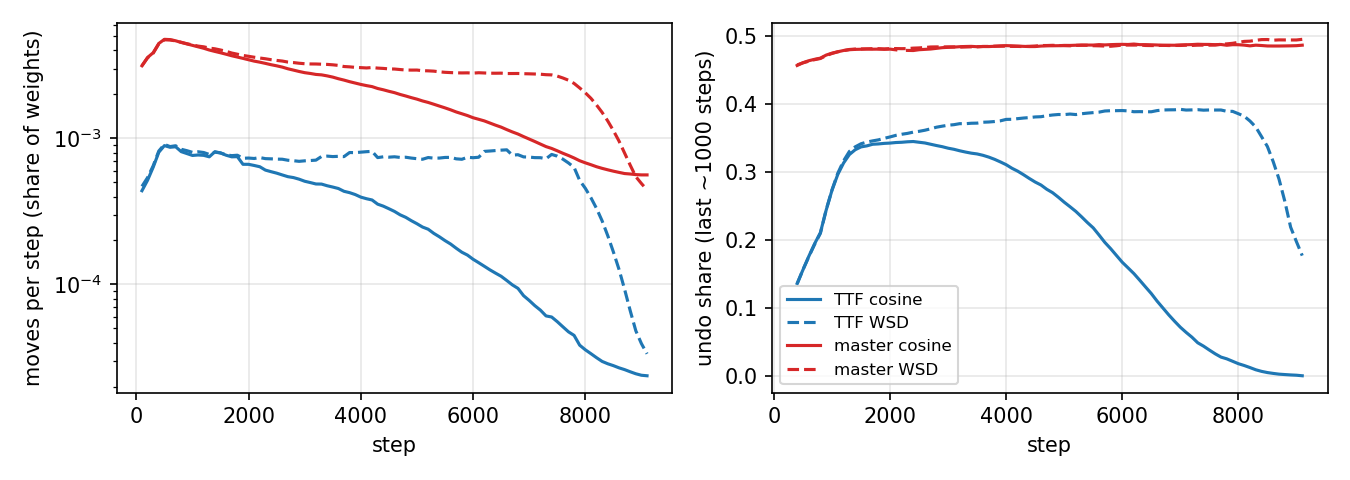
\includegraphics[width=\linewidth]{figures/wsd_movediag_small.png}
\caption{Trit moves under cosine and WSD (110M, 9155 steps, rank 512). Left: moves per step (share of weights). Right:
share of moves that undo the net change of the last $\sim$1000 steps. TTF under WSD keeps moving and undoing at the peak
step until the decay, which is too short to reach the cosine's late regime; master's moves are half undone under both.}
\label{fig:wsdmoves}
\end{figure}

\subsection{Is TTF a low-rank Adam with a straight-through estimator?}\label{sec:lowrankste}
Both keep $O(r(N+K))$ optimizer numbers per layer and both read the gradient through the ternary forward. In the low-rank
STE the \emph{latent} is low rank, so every change the network can make to a layer lies in a rank-$r$ subspace around a
fixed random initialisation. In TTF the low-rank object is only the \emph{evidence since the last move}. A move is
written into the full-rank trits and the evidence is spent. At rank 512, the low-rank STE at its best learning rate
(5e-4) ends at 2.8867, which is 0.21 behind TTF (Table~\ref{tab:110m}). Higher learning rates are worse or diverge.

\subsection{Scale}

\begin{table*}[t]
\centering
\caption{Scale (fixed windows; Wikipedia / FineWeb-Edu). Master + extras at its best learning rate. 1.3B and 2.9B TTF use
$p=0.5$; 340M rank runs use the final recipe.}
\label{tab:scale}
\resizebox{\linewidth}{!}{\begin{tabular}{llrrr}
\toprule
size & method (numbers of state per weight) & Wikipedia & FineWeb-Edu & $\Delta$ \\
\midrule
340M & master + extras (lr 1e-3, 2 seeds) & 2.5878 & 3.5458 & \\
     & TTF with momentum, rank 512 (2 seeds) & 2.5770 & 3.5251 & $-0.011$ / $-0.021$ \\
     & TTF, rank 64 (0.10) & 2.8142 & 3.7961 & $+0.226$ / $+0.250$ \\
     & TTF, rank 128 (0.20) & 2.7175 & 3.6858 & $+0.130$ / $+0.140$ \\
     & TTF, rank 256 (0.39) & 2.6246 & 3.5800 & $+0.037$ / $+0.034$ \\
     & TTF, rank 512 (0.79) & 2.5563 & 3.5039 & $-0.032$ / $-0.042$ \\
     & TTF, full rank 1024 (1.57) & \textbf{2.5167} & \textbf{3.4584} & $\mathbf{-0.071}$ / $\mathbf{-0.087}$ \\
1.3B & master + extras (lr 5e-4) & 2.4796 & 3.4344 & \\
     & TTF, rank 128 (0.10), $p=0.75$ + annealed leak & 2.6464 & 3.6169 & $+0.167$ / $+0.183$ \\
     & TTF, rank 256 (0.20), $p=0.75$ + annealed leak & 2.5654 & 3.5226 & $+0.086$ / $+0.088$ \\
     & TTF, rank 512 (0.39) & 2.5012 & 3.4415 & $+0.022$ / $+0.007$ \\
     & TTF, rank 1024 (0.79) & 2.4742 & 3.4153 & $-0.005$ / $-0.019$ \\
     & \quad seed 2 (master seed 2: 2.4807 / 3.4374) & 2.4656 & 3.4031 & $-0.014$ / $-0.031$ \\
     & TTF, full rank 2048 (1.57), $p=0.75$ + annealed leak & \textbf{2.4289} & \textbf{3.3654} & $\mathbf{-0.051}$ / $\mathbf{-0.069}$ \\
     & TTF, rank 512, $p=0.75$ + annealed leak & 2.4999 & 3.4463 & $+0.020$ / $+0.012$ \\
2.9B (FineWeb-Edu) & master (lr 4e-4) & 3.1220 & 2.8911 & \\
     & TTF, rank 1024 (0.55) & 3.1391 & 2.9005 & $+0.017$ / $+0.009$ \\
     & TTF, rank 1536 (0.79) & 3.1243 & \textbf{2.8867} & $+0.002$ / $\mathbf{-0.004}$ \\
     & TTF, rank 512 (0.28), steps 1000 / 2000$^\ddagger$ & & 3.998 / 3.617 & $-0.028$ / $+0.007$ \\
\bottomrule
\multicolumn{5}{l}{\footnotesize $^\ddagger$ training-time validation at matched steps (run stopped at the end of the
booking); rank 1024 / 1536 / master: 3.956 / 3.944 / 4.026 at 1000, 3.577 / 3.568 / 3.610 at 2000.}
\end{tabular}}
\end{table*}

TTF leads master + extras by 0.044 at 110M and by 0.032 at 340M at rank 512 (0.071 at full rank). At 1.3B and 2.9B
it is level when the state is about 0.8 numbers per weight, and behind at about half that (Table~\ref{tab:scale}). A
different schedule does not make up for the rank. At 1.3B and rank 512 the final recipe ($p=0.75$, annealed leak) ends
where $p=0.5$ does ($-0.001$). With a second seed of both 1.3B arms, TTF at rank 1024 leads by 0.010 over the two seeds.
TTF's seeds differ by 0.009 and master's by 0.001, and each TTF seed is ahead of each master seed on both sets.

\subsection{Training length}\label{sec:depth15}
The budgets above are far below compute-optimal for 340M and larger. To see whether the ternary gap grows as training
gets longer, we trained a 15M model (14.6M parameters, width 256, 8 blocks, tied 32k embedding) from scratch in full
precision and with TTF on the same 2.0B-token FineWeb-Edu stream. Training windows are sampled at random, so the longest
budget draws 1.5B tokens and sees about half of the stream's windows. Each method ran once at a constant learning rate
(the stable phase of a warmup--stable--decay schedule). Branches taken at 90\% of each budget cooled down to the minimum
learning rate at 300M, 600M and 1.5B tokens, which is 1, 2 and 5 times the compute-optimal 20 tokens per parameter
\citep{hoffmann2022chinchilla}, counting all parameters. TTF uses the scratch recipe ($\theta=16$, full rank at this
width, row and column scales and rank-16 float adapters), full precision the same learning rate (1.5e-3) without them.
Every branch end is scored on the same fixed windows (Table~\ref{tab:depth15}). From 300M to 1.5B tokens full precision
gains 0.172 and TTF 0.175, so the gap on FineWeb-Edu stays at 0.11. On Wikipedia it grows from 0.075 to 0.095 and then
holds. Over this range, the gap between a ternary network and its full-precision twin trained on the same tokens does
not grow with training. The test covers one size, one run per point and one learning rate for both precisions, so we do
not extrapolate the flat gap beyond this range.

\begin{table}[t]
\caption{Training length and the ternary gap: a 15M model trained from scratch in full precision and with TTF (the
scratch recipe, $\theta=16$) on the same FineWeb-Edu stream, cooldown branches at 1, 2 and 5 times compute-optimal
(20 tokens per parameter). Fixed windows: the first 2000 of FineWeb-Edu validation (the scores shown), the 974 of
Wikipedia validation.}
\label{tab:depth15}
\resizebox{\linewidth}{!}{\begin{tabular}{lrrrr}
\toprule
tokens (per parameter) & full precision & TTF & gap FineWeb-Edu & gap Wikipedia \\
\midrule
300M (21) & 3.4949 & 3.6097 & $+0.115$ & $+0.075$ \\
600M (41) & 3.4057 & 3.5145 & $+0.109$ & $+0.095$ \\
1.5B (103) & 3.3232 & 3.4346 & $+0.111$ & $+0.093$ \\
\bottomrule
\end{tabular}}
\end{table}

\section{The size of the state}\label{sec:rank}
The size of TTF's state is set by the rank of its accumulators.

\paragraph{One curve across sizes.} Figure~\ref{fig:rank} plots TTF minus master against the numbers of state per
weight. At 1.3B (Wikipedia) and 2.9B (FineWeb-Edu) the four points lie on one line,
\begin{equation}
  \Delta \approx -0.014 - 0.027\,\log_2(\text{numbers per weight}),
\end{equation}
with a residual of 0.0005 on fixed windows. Fitted separately, the slope is $-0.0270$ per doubling at 1.3B and $-0.0271$
at 2.9B, with break-even at 0.68 and 0.70. Each doubling of the state is worth 0.027, and TTF reaches master at about
0.70 numbers per weight. That is 1.05 bytes at 12 bits, against 12 bytes for master and 4 for the one-float master.

\begin{table}[t]
\caption{110M rank sweep on the final recipe (fixed windows, Wikipedia; master + extras 2.7166, two seeds).}
\label{tab:rank110}
\resizebox{\linewidth}{!}{\begin{tabular}{rrrr}
\toprule
rank & numbers per weight & Wikipedia & $\Delta$ \\
\midrule
64 & 0.13 & 2.9458 & $+0.229$ \\
128 & 0.27 & 2.8410 & $+0.124$ \\
192 & 0.40 & 2.7774 & $+0.061$ \\
256 & 0.53 & 2.7389 & $+0.022$ \\
384 & 0.79 & 2.6975 & $-0.019$ \\
512 & 1.06 & 2.6728 & $-0.044$ \\
768 (full) & 1.59 & 2.6480 & $-0.069$ \\
\bottomrule
\end{tabular}}
\end{table}

At 110M we trained seven ranks on the final recipe, from 64 to full (Table~\ref{tab:rank110}). This curve is steeper
and bent. It falls by about 0.10 per doubling below half a number per weight, 0.07 around one and 0.04 above it (a
quadratic in $\log_2$ fits to 0.004). It crosses master at 0.67 numbers per weight, close to where the 1.3B and 2.9B
lines cross (Figure~\ref{fig:rank}).

\paragraph{Where the sizes agree, and where they do not.} The break-even state is about the same at all four sizes: 0.67
numbers per weight at 110M, 0.57 at 340M (between ranks 256 and 512), 0.68 at 1.3B and 0.70 at 2.9B. That is a rank of
0.36--0.45 of the width. A model needs about this share of state to match master, whatever its size. The cost of going
below it differs. At 0.39--0.40 numbers per weight, 110M trails master by 0.061, 340M by 0.037 and 1.3B by 0.022.
Between 0.4 and 0.8 numbers per weight, 110M gains 0.08 per doubling, 340M 0.07, and 1.3B and 2.9B 0.027. Below 0.4 the
1.3B curve steepens too (0.066 from 0.20 to 0.39). Above break-even the smaller models also gain more. At full rank TTF
leads by 0.069 at 110M, 0.071 at 340M and 0.051 at 1.3B. The larger models' gap is flatter on both sides, with less to
lose from a small state and less to win from a large one.

\begin{table}[t]
\caption{Cost of halving the rank: the loss difference between neighbouring ranks (fixed windows, Wikipedia). 1.3B:
the final recipe up to rank 512, $p=0.5$ for $512\to1024$. 2.9B: FineWeb-Edu, the $1024\to1536$ step (0.014) scaled to a
full halving.}
\label{tab:halving}
\resizebox{\linewidth}{!}{\begin{tabular}{lrrrr}
\toprule
ranks & 110M & 340M & 1.3B & 2.9B \\
\midrule
$64\to128$ & 0.105 & 0.097 & & \\
$128\to256$ & 0.102 & 0.093 & 0.081 & \\
$256\to512$ & 0.066 & 0.068 & 0.066 & \\
$512\to1024$ & & 0.040$^*$ & 0.027 & \\
$1024\to1536$ & & & & 0.024 \\
\midrule
first halving below full rank & 0.050 & 0.040 & 0.045 & \\
full rank against master & $-0.069$ & $-0.071$ & $-0.051$ & \\
\bottomrule
\multicolumn{5}{l}{\footnotesize $^*$ ends at full rank.}
\end{tabular}}
\end{table}

\paragraph{A share of the weights, or a rank?} For the 1.3B and 2.9B models the state per weight is proportional to rank /
width, because the shapes are alike, so these points alone cannot tell whether the rank needed scales with width. Three
comparisons can. First, a fixed rank that leads master at one width trails it at another. At rank 1024 the gap is
$-0.071$ at 340M (width 1024), $-0.005$ at 1.3B (2048) and $+0.009$ at 2.9B (3072). At rank 512 it is $-0.044$ at 110M,
$-0.032$ at 340M and $+0.022$ at 1.3B. Second, at a fixed share the sign of the gap is the same at every size, and its
size shrinks with the model. At 0.79 numbers per weight the gap is $-0.019$, $-0.032$, $-0.005$ and $-0.004$ at 110M,
340M, 1.3B and 2.9B, and at 0.39--0.40 it is $+0.061$, $+0.037$ and $+0.022$. Third, a halving of the rank costs the same
at 110M and 340M at the same absolute rank, and the same again at 1.3B for $256\to512$ at twice the width
(Table~\ref{tab:halving}). It does not cost the same at the same share. A fit over all sizes and ranks,
$L = L_\infty + c\,(w/768)^{gb}(r^{-b} - w^{-b})$, puts the width exponent at $g=-0.67$ (68\% interval $-0.8$ to $-0.6$).
The state that keeps the rank cost fixed therefore grows more slowly than the weights.

Both readings hold because the full-rank lead over master shrinks with size. The rank sets the loss that a given rank
costs, and the share sets the rank at which TTF meets master. The cost per halving falls with the rank, and at a fixed
share it falls with the size, down to 0.027 between ranks 512 and 1024 at 1.3B and 0.024 per halving between 1024 and
1536 at 2.9B. The state does not have to grow with the weights to keep its cost.

\begin{table*}[t]
\centering
\caption{Gradient spectra at step 4000 (Wikipedia; 2.9B on FineWeb-Edu). Top: share of a step's normalised energy kept by
the top-$r$ subspace of the mean gradient. Middle: share dropped by halving the rank from $r$, the real step against the
covariance model. Bottom: energy of the gradient that persists over 1000 steps, left outside ranks of 1/8, 1/4 and 1/2
of the width.}
\label{tab:spectra}
\begin{tabular}{lrrrrr}
\toprule
\multicolumn{6}{l}{\emph{kept at rank $r$}} \\
$r$ & 64 & 128 & 256 & 512 & 1024 \\
110M & 0.44 & 0.59 & 0.76 & 0.92 & \\
340M, earlier recipe & 0.43 & 0.58 & 0.74 & 0.89 & \\
340M, final recipe & 0.38 & 0.54 & 0.70 & 0.87 & \\
1.3B & 0.34 & 0.48 & 0.64 & 0.79 & 0.91 \\
2.9B & 0.31 & 0.45 & 0.61 & 0.76 & 0.88 \\
\midrule
\multicolumn{6}{l}{\emph{dropped by halving from $r$, real / model}} \\
$r$ & 16 & 32 & 64 & 128 & 256 \\
110M & 0.137 / 0.144 & 0.156 / 0.169 & 0.147 / 0.163 & 0.113 / 0.126 & 0.061 / 0.066 \\
340M & 0.129 / 0.131 & 0.158 / 0.163 & 0.163 / 0.169 & 0.137 / 0.143 & 0.083 / 0.086 \\
\midrule
\multicolumn{6}{l}{\emph{persistent energy outside a share of the width}} \\
share & 1/8 & 1/4 & 1/2 & & \\
340M & 0.279 & 0.127 & 0.032 & & \\
1.3B & 0.200 & 0.081 & 0.018 & & \\
2.9B & 0.166 & 0.062 & 0.015 & & \\
\bottomrule
\end{tabular}
\end{table*}

\paragraph{Why a halving costs what it does.} At step 4000 of the 110M, 340M and 1.3B runs (Wikipedia, and at 1.3B every
fourth ternary layer) we measured each layer's normalised gradient $u=g/\sqrt v$, with the checkpoint's factored $v$, for
single training batches, and its mean over 192 micro-batches of 4 sequences. Four measurements together account for the
cost of a halving.

\emph{A step spreads its energy evenly over octaves of directions.} Each halving of the rank drops 0.14--0.17 of a
step's $\|u\|^2$ (Table~\ref{tab:spectra}, top), at every width and at every rank up to half the width. Singular values
whose squares fall as $1/k$ would do exactly this.

\emph{The dropped energy is worth less at higher rank, the same at every width.} Dividing the cost of a halving by the
energy it drops gives 0.58--0.67 between ranks 64 and 256 (110M, 340M), 0.41--0.47 between 256 and 512 (110M, 340M,
1.3B) and 0.22 between 512 and 1024 at 1.3B. The cost of a halving is the product of the two factors, for example
$0.15\times0.44\approx0.066$ between ranks 256 and 512, and neither factor depends on the width. This is why the cost
follows the absolute rank. We measured both factors rather than derived them, and both belong to the data at 32k tokens
per step. The batch sets a step's spectrum and could change them, but in our tests it does not
(Appendix~\ref{app:variants}).

\emph{A small state holds the part of the gradient that lasts.} The energy of the mean gradient that is consistent
across independent batches (cross products of thirds) lies 4.9\%, 4.2\% and 8.9\% outside rank 128 at 110M, 340M and
1.3B, and 0.2\%, 0.3\% and 1.5\% outside rank 512. Legal moves chosen from its rank-$r$ truncation (the top 0.1\% or 1\%
by size) and scored on independent batches gain as much as the full-rank choice, and 2--7\% more at ranks 32--128,
because truncation removes selection noise. What a small state loses is therefore not this direction. It loses the part
of each step that is real and short-lived. The mean gradient turns within the accumulator's memory (cosine 0.3--0.5
between steps 4000 and 5000 at 1.3B, depending on depth, and 0.25--0.65 at 2.9B), and a full-rank accumulator integrates
every entry's share of it. The moves in Appendix~\ref{app:variants} agree. Low-rank moves land on different entries, and
matching the full-rank move count does not improve the loss. So do the changes that failed there. A shorter memory ($\tau=300$ at
rank 128, $+0.060$) forgets the lasting part sooner, and neither a basis refresh nor a sketch can hold an evenly spread
step in fewer directions. Only feeding the discarded part back densely helped.

\emph{Low rank also makes fewer moves.} Over steps 1500--2500 at 110M the moves per step are 0.015\%, 0.047\%, 0.067\%
and 0.086\% of the weights at ranks 64, 256, 512 and full, and 58\%, 21\%, 14\% and 13\% of the weights never move. At
340M, ranks 64, 128 and 512 make 0.013\%, 0.023\% and 0.058\%.

\paragraph{Why break-even falls at a share.} Full-rank TTF leads master by about the same amount at every size, and the
first halving below full rank costs about as much (Table~\ref{tab:halving}, lower block). At every size TTF therefore
reaches master about one halving below full rank, and a halving is defined by the width. Break-even sits at a share of
the width because both the lead and the cost of the first halving are roughly constant in loss across sizes. That first
halving costs more than the absolute-rank trend predicts. At 1.3B, $2048\to1024$ costs 0.045 against 0.027 for
$1024\to512$, and at 340M $1024\to512$ costs 0.040 against 0.027 at 1.3B.

This is not a premium for having no projection at all. At 340M, after a third of the training, ranks 512, 896 and 1024
end at 2.9215, 2.8869 and 2.8787. Rank 896 is 0.19 halvings below full and 0.0082 behind it, where a straight line in
$\log r$ between 512 and full puts it (0.0083). At 110M, rank 704 likewise sits on the trend (3.0128, against 3.0339 at
512 and 3.0107 at full), and spending exactly at the moved entries recovers none of the gap at rank 512 ($-0.002$). The
last halving is steeper, smoothly in $\log r$. The part of the gradient that is consistent across batches points
the same way. At 1.3B its energy outside rank $2r$ equals 340M's outside rank $r$ (0.089, 0.042, 0.015 and 0.003 at
ranks 128--1024 against 64--512), and at least 98.5\% of it is held at about half the width. This comparison uses an
earlier 340M recipe and the consistency within one checkpoint.

\paragraph{The input spectrum sets the share a halving drops.} One step's gradient is $\sum_t\delta_tx_t^\top$ over the
batch's tokens. We built a random matrix from only the measured input covariance $C_x=\sum x x^\top$ and error
covariance $C_\delta=\sum\delta\delta^\top$ of one batch, $C_\delta^{1/2}ZC_x^{1/2}$ with $Z$ i.i.d.\ Gaussian and the
same $\sqrt v$ normalisation. It reproduces the kept share of the real step at every rank (Table~\ref{tab:spectra},
middle). The eigenvalues of the input covariance fall as $\lambda_i\propto i^{-1}$ in every layer type (fitted slopes
$-0.95$ to $-1.17$, and $-0.5$ to $-1.3$ for the errors). That is an equal share of variance per octave of directions,
so each halving of the rank drops about the same share of a step until the rank nears the end of the spectrum. Neither
the width nor the batch enters in our measurements.

\paragraph{The persistent gradient grows with the width.} On the final recipe at 340M (snapshots at steps 4000 and 5000,
measured as at 1.3B and 2.9B), a halving also drops 0.16--0.17 of a step's energy, so the per-halving share holds at
every width. At the same rank the narrower model keeps somewhat more of a step (0.38, 0.34 and 0.31 at rank 64 for
340M, 1.3B and 2.9B), as if the rank grew as about $d^{0.3}$. The gradient that persists over 1000 steps (cross products
of independent means) follows neither the rank nor the share (Table~\ref{tab:spectra}, bottom). At a fixed share it
shrinks with the width, and at a fixed rank it grows (outside rank 512: 0.032, 0.081 and 0.116 at 340M, 1.3B and 2.9B).
Matching the levels needs a rank that grows as about $d^{0.5}$ between 340M and 1.3B (both on Wikipedia) and $d^{0.65}$
between 1.3B and 2.9B (FineWeb-Edu at 2.9B, with slightly different recipes). Most of the first exponent comes from the
recipe. On one recipe and one data set ($p=0.5$ on Wikipedia, 110M against 1.3B, snapshots at steps 4000 and 5000), the
levels 0.20, 0.081 and 0.037 are left outside ranks of about 92, 205 and 323 at width 768, and of 256, 512 and 768 at
width 2048. That is a rank growing as $d^{0.9}$ to $d^{1.05}$, close to a fixed share of the width.

The absolute rank therefore sets most of what a low-rank state loses step by step, while the part that the lead over
master needs grows with the width, more slowly than the width itself. Break-even at about one halving below full rank
is what we measured at every size, and this split is our reading of it.

\paragraph{How much can be saved.} At break-even the state is 1.05 bytes per weight at 12 bits, 11 times less than
master's 12. Halving it to 0.35 numbers per weight (0.5 bytes, 23 times less) costs about 0.03 at 1.3B and 2.9B and
about 0.08 at 110M. Quartering it costs 0.05 at the larger sizes (extrapolated) and 0.19 at 110M. In the sense that
matters, the loss is sublinear in the state. Each halving costs a fixed amount at 1.3B and 2.9B, not a fixed fraction
of what is left, so the first halvings below break-even are cheap at scale.

\begin{figure*}[t]
\centering
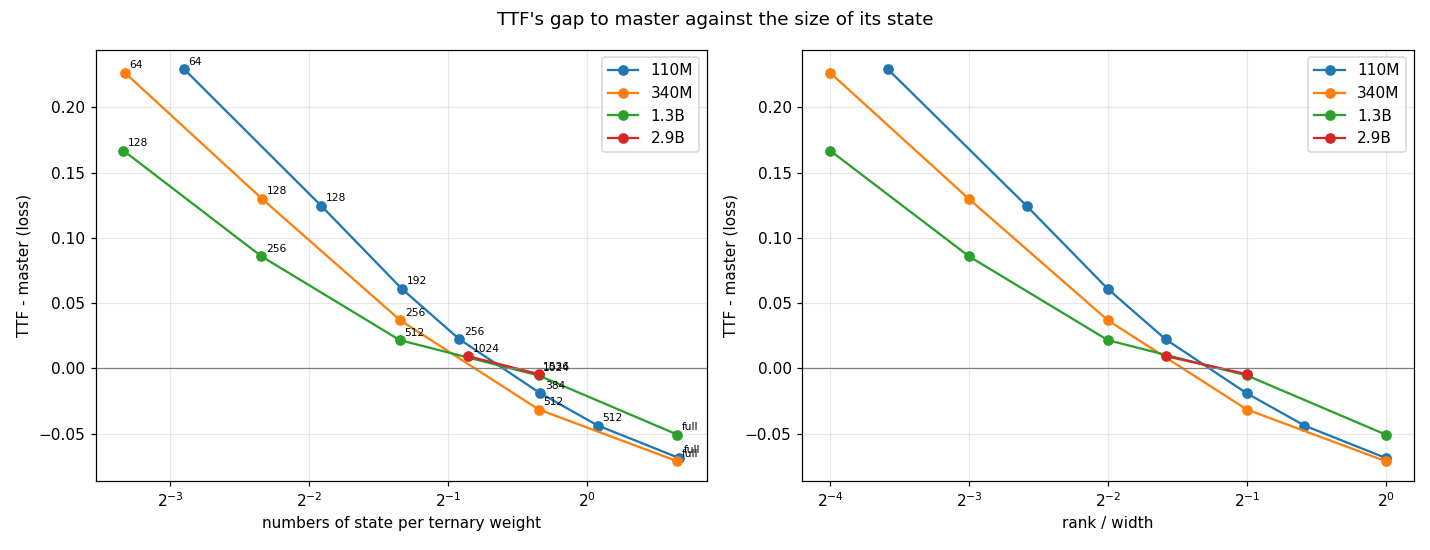
\includegraphics[width=\linewidth]{figures/rank_curve.png}
\caption{TTF minus master (fixed windows) against the optimizer state per ternary weight (left) and against rank / width
(right). 110M and 340M: final recipe, ranks 64--full; 1.3B: ranks 128 / 256 / full ($p=0.75$ + annealed leak), 512 / 1024 ($p=0.5$); 2.9B: ranks 1024 / 1536. All four
cross master at 0.57--0.70 numbers per weight.}
\label{fig:rank}
\end{figure*}

\subsection{Getting more from a small state}\label{sec:adaptive}
A fixed amount of state can be spent better in three ways, and one obvious adjustment does not help.

\emph{Precision for rank.} Since the accumulator tolerates 12 bits, a budget is better spent on rank than on precision.
At the bytes of rank 128 in fp32, rank 340 with a 12-bit accumulator ends at 2.7086 against 2.8410 for rank 128, which
is $-0.132$ for the same memory ($-0.149$ on FineWeb-Edu). Interpolating between fp32 ranks 256 and 384 (2.7389 and
2.6975) puts rank 340 at 2.710, so 12-bit storage leaves the loss unchanged at this rank too. Rank 340 is 0.008 ahead of master + extras
(2.7166), which puts break-even at 1.05 bytes of state per weight.

\emph{Rank where the energy is.} Under a fixed budget $B=\sum_l r(N_l+K_l)$ we reallocate the rank every 500 steps. Each
layer's singular values $s_i$ of $UV^\top$ (those of $U$, since $V$ is orthonormal) are priced by energy per stored
number, $s_i^2/(N_l+K_l)$. One global threshold keeps the directions above it, a layer whose every direction is above it
grows by a quarter, and ranks move by at most 25\% per reallocation. At 340M with the rank-256 budget, adaptive ranks
end at 2.6121, against 2.6246 for a fixed rank 256 ($-0.013$ for the same state, $-0.011$ on FineWeb-Edu) and 2.5563 for
a fixed rank 512. That is about a fifth of the way from one to the other. The budget moves to the MLP (final ranks q
157, k 143, v 150, o 177, gate 313, up 321, down 346), so the MLP matrices, $2.75\times$ wider, get about twice the rank.

\emph{Rank over time.} At 110M a rank growing linearly from 512 to 768 (average 640) ends at 2.6573, 0.016 ahead of a
fixed rank 512 (2.6728) and 0.009 behind a fixed rank 768 (2.6480). That is about what its average rank buys at a fixed
rank. At 340M, a rank growing from 128 to 384 (average 256) ends at 2.6301, against 2.6246 at a fixed rank 256 and 2.7175
at a fixed rank 128, again what the average rank buys. A growing rank ends where a fixed rank at its average ends, neither
better nor worse.

\emph{A shorter memory at low rank does not help.} A rank-128 accumulator with $\tau=300$ instead of 1000 ends at 2.9008,
0.060 behind (0.073 on FineWeb-Edu). A small basis does not need to forget faster.

\paragraph{Rank is also compute.} On one RTX 4070 Ti Super (batch $16\times2048$, steps 10--50), a TTF step at 110M
takes 1.83, 1.85, 1.90, 1.99 and 2.07 s at ranks 64, 128, 256, 512 and 768, against 1.88 s for master. At 340M it takes
4.92, 5.05, 5.27 and 5.68 s at ranks 128, 256, 512 and 1024, against 5.02 s. Rank costs at most 15\% of step time over
a twelvefold range of ranks, and near the break-even state a TTF step takes 3--9\% longer than master's. At these sizes
peak GPU memory is set by the activations (7.0--7.5 GiB for TTF and 4.8 for master at 110M, 11.0--12.5 against
10.3 at 340M), not by the optimizer state (43 MiB to 1.8 GiB for TTF). Section~\ref{sec:memory} measures the regime where the
state dominates.

\section{Training dynamics of threshold flips}\label{sec:dynamics}

In master, a smaller learning rate makes every latent step smaller and the noise of the update falls with it. In TTF the
move size is fixed at one level, and the step scale only changes \emph{how often} weights move. All at 110M, rank 512.

\subsection{A freeze under a decaying step with a constant leak}
With a constant leak the accumulator of a weight with mean normalised drift $m$ settles near $\tau a m$, while its noise
is about $a\sigma\sqrt{\tau/2}$. Both scale with $a$, but the threshold does not. As $a$ falls, the barrier between the
settled evidence and $\theta$ grows like $1/a$, and the move rate falls exponentially. With $p=1$ moves per step fall from
$3\times10^{-4}$ to $5\times10^{-9}$ between $\rho=0.67$ and $\rho=0.10$, while master's trit changes fall only
fourfold. Fitted as a power of $\rho$ over steps 4000--8000, the move rate falls as $\rho^{0.78}$ for master,
$\rho^{1.25}$ for TTF with $p=0.5$, and $\rho^{4.4}$ with $p=1$. So $p=1$, which leads by 0.05 at mid-training, ends
0.025 behind $p=0.5$. Rank, spend and the leak itself are not the cause. Full rank behaves the same, and no leak is
worse.

\paragraph{Annealing the leak with the step.} With $\lambda_s=a_s$ the memory grows as the step falls, the settled
evidence is $\tau m$ independent of $a$, and the noise in $A$ shrinks as $\sqrt a$, so the barrier no longer grows. With
$p=1$ the annealed leak keeps the mid-training lead ($-0.040$ at step 6000) and keeps weights moving
($8\times10^{-6}$ per step at the end instead of $5\times10^{-9}$). It ends level with $p=0.5$ ($+0.004$ and $+0.008$ for
two seeds). $p=0.75$ with the annealed leak is $-0.021$ at mid-training and level at the end (2.6728 vs 2.6720), and leads by
0.019 at twice the tokens (FineWeb-Edu 3.0423 vs 3.0616).

\subsection{Fewer moves late in training, each worth more}\label{sec:late}
TTF's progress per step slows in the last third of training, and the colder schedules hand back part of their mid-run
lead (Table~\ref{tab:lategap}). At $p=0.5$, full rank gains 0.026 on master after step 6000 and rank 512 gains 0.017,
while at $p=1$ both lose ground. We measured what the moves are worth.

\begin{table}[t]
\caption{TTF minus master at step 6000 and at the end (110M, training-time).}
\label{tab:lategap}
\resizebox{\linewidth}{!}{\begin{tabular}{lrr}
\toprule
TTF & step 6000 & end \\
\midrule
rank 512, $p=0.5$ & $-0.026$ & $-0.043$ \\
rank 512, $p=0.75$ + annealed leak & $-0.047$ & $-0.041$ \\
rank 512, $p=1$ + annealed leak & $-0.066$ & $-0.038$ \\
full rank, $p=0.5$ & $-0.042$ & $-0.068$ \\
full rank, $p=1$ + annealed leak & $-0.086$ & $-0.064$ \\
\bottomrule
\end{tabular}}
\end{table}

\paragraph{Measuring a move.} Every 100 steps, around the real training step and on fixed probe batches, we record the
moves of this step, their first-order gain on a true gradient (dL/dT from 8 batches, and for master the STE gradient times
$\gamma$), and the share that goes downhill (the precision). We also measure the value of the last $\sim$1000 steps of
moves by putting the trits of 1000 steps ago back in with today's float parameters. A move's value can show only after
the floats adapt to it, and the one-step loss change is too noisy ($\pm3\times10^{-3}$).

\begin{table*}[t]
\centering
\caption{What a step of trit moves is worth (110M; means over phases of training). Moves per step over the window;
net / gross: entries changed over the last $\sim$1000 steps over the moves made in them; value per step: the loss the
last $\sim$1000 steps of moves are worth (their trits put back), per step; value per move: the same over the moves.}
\label{tab:late}
\resizebox{\linewidth}{!}{\begin{tabular}{llrrrrr}
\toprule
 & steps & moves per step & net / gross & value per step & value per move & precision \\
\midrule
master & 3000--5000 & 221k & 0.08 & $1.6\times10^{-4}$ & $7.2\times10^{-10}$ & 0.522 \\
       & 7000--9155 & 70k & 0.09 & $4.3\times10^{-5}$ & $6.0\times10^{-10}$ & 0.518 \\
TTF $p=0.5$ & 3000--5000 & 45k & 0.55 & $2.0\times10^{-4}$ & $4.5\times10^{-9}$ & 0.523 \\
       & 7000--9155 & 8.7k & 0.91 & $6.9\times10^{-5}$ & $8.5\times10^{-9}$ & 0.506 \\
TTF $p=0.75$ + ann. & 3000--5000 & 40k & 0.58 & $2.2\times10^{-4}$ & $5.6\times10^{-9}$ & 0.521 \\
       & 7000--9155 & 4.9k & 0.96 & $6.4\times10^{-5}$ & $1.4\times10^{-8}$ & 0.512 \\
\quad rank 128 & 3000--5000 & 15k & 0.69 & $2.0\times10^{-4}$ & $1.3\times10^{-8}$ & 0.528 \\
       & 7000--9155 & 1.6k & 0.85 & $4.8\times10^{-5}$ & $3.0\times10^{-8}$ & 0.512 \\
\quad full rank & 3000--5000 & 51k & 0.44 & $2.2\times10^{-4}$ & $4.3\times10^{-9}$ & 0.522 \\
       & 7000--9155 & 6.5k & 0.94 & $6.3\times10^{-5}$ & $1.0\times10^{-8}$ & 0.514 \\
\bottomrule
\end{tabular}}
\end{table*}

The slowdown is in the number of moves, not in their quality (Table~\ref{tab:late}, Figure~\ref{fig:movediag}). From
mid to late training TTF's moves per step fall eightfold ($p=0.75$) while the value of each move rises
2.4-fold, while master's moves fall threefold while the value of each falls slightly. Precision, the share of moves that go
downhill, falls slightly for both (0.52 to 0.51--0.52). Late in training TTF's moves are worth more per step than
master's ($6.4$--$6.9\times10^{-5}$ against $4.3\times10^{-5}$), with 8--14 times fewer of them.

Master's extra moves are back-and-forth. Over 1000 steps only 8--9\% of master's trit changes survive as net change.
Its latents dither across cell boundaries, and 48\% of its changes at any step reverse the net change of the last 1000
steps.
TTF's moves mostly stay (net over gross 0.55--0.6 mid-training, 0.9--0.96 late), because a spent move must re-earn
$\theta$ of evidence before it can reverse whereas the master can cross back with an arbitrarily small step. Per \emph{net} change, TTF's late moves are worth about twice master's
($1.4\times10^{-8}$ against $6.8\times10^{-9}$).

The late schedule sits at a trade-off rather than being stuck. Raising the late step scale by lowering $p$ to 0.5 from
step 6000 costs 0.012, and lowering it to 0.25 costs 0.068. Raising the threshold from step 6000 to 20, 24 or 32, for
fewer and stronger moves, is ahead by 0.005--0.012 at step 7000 and behind at the end (by 0.001, 0.004 and 0.013).
Freezing the trits at step 4000, 6000 or 8000 gains 0.031, 0.011 or 0.001 in the next 250 steps, because the disturbance
of ongoing moves falls to almost nothing, and loses 0.048 (frozen from 6000) or 0.009 (from 8000) by the end. Late moves
are progress, and the marginal move is worth what it costs in both directions. The shape of the decay matters little.
The shared learning-rate schedule sets both the float tail's steps and TTF's step scale. A linear decay to the same
floor gives 2.6768, a linear decay to zero 2.6786 and a floor three times lower (4.5e-5) 2.6774, all against 2.6728 for
the cosine (seed 2: 2.6671) and so within seed noise. Only a floor three times higher (4.5e-4) costs 0.044 (2.7168).

\paragraph{Rank does not cause the slowdown above rank 512.} With the same schedule ($p=0.75$, annealed leak), full
rank makes a third more late moves than rank 512, each worth less, for the same value per step (Table~\ref{tab:late}).
Mid-training, ranks 128, 512 and full earn almost the same. Only the smallest state limits late progress. At rank 128
fewer weights reach the threshold and the late value is 25\% lower. Above that, the schedule and not the state sets the
late slowdown, and more state late in training cannot fix it. A rank grown over training ends where its average rank
would (Section~\ref{sec:adaptive}).

\paragraph{The schedule is part of the method.} If late progress is a long run of rare, valuable moves, a schedule that
holds the step high and decays only at the end should suit TTF worse than a cosine, and master better. It does
(Section~\ref{sec:results}): at 600M tokens WSD costs TTF 0.054 and gains master 0.010. TTF should be run with a long
decay, and a WSD decay over the last 50\% matches the cosine (Table~\ref{tab:sched}). We measure TTF's lead over master
at each method's better schedule.

\begin{figure}[t]
\centering
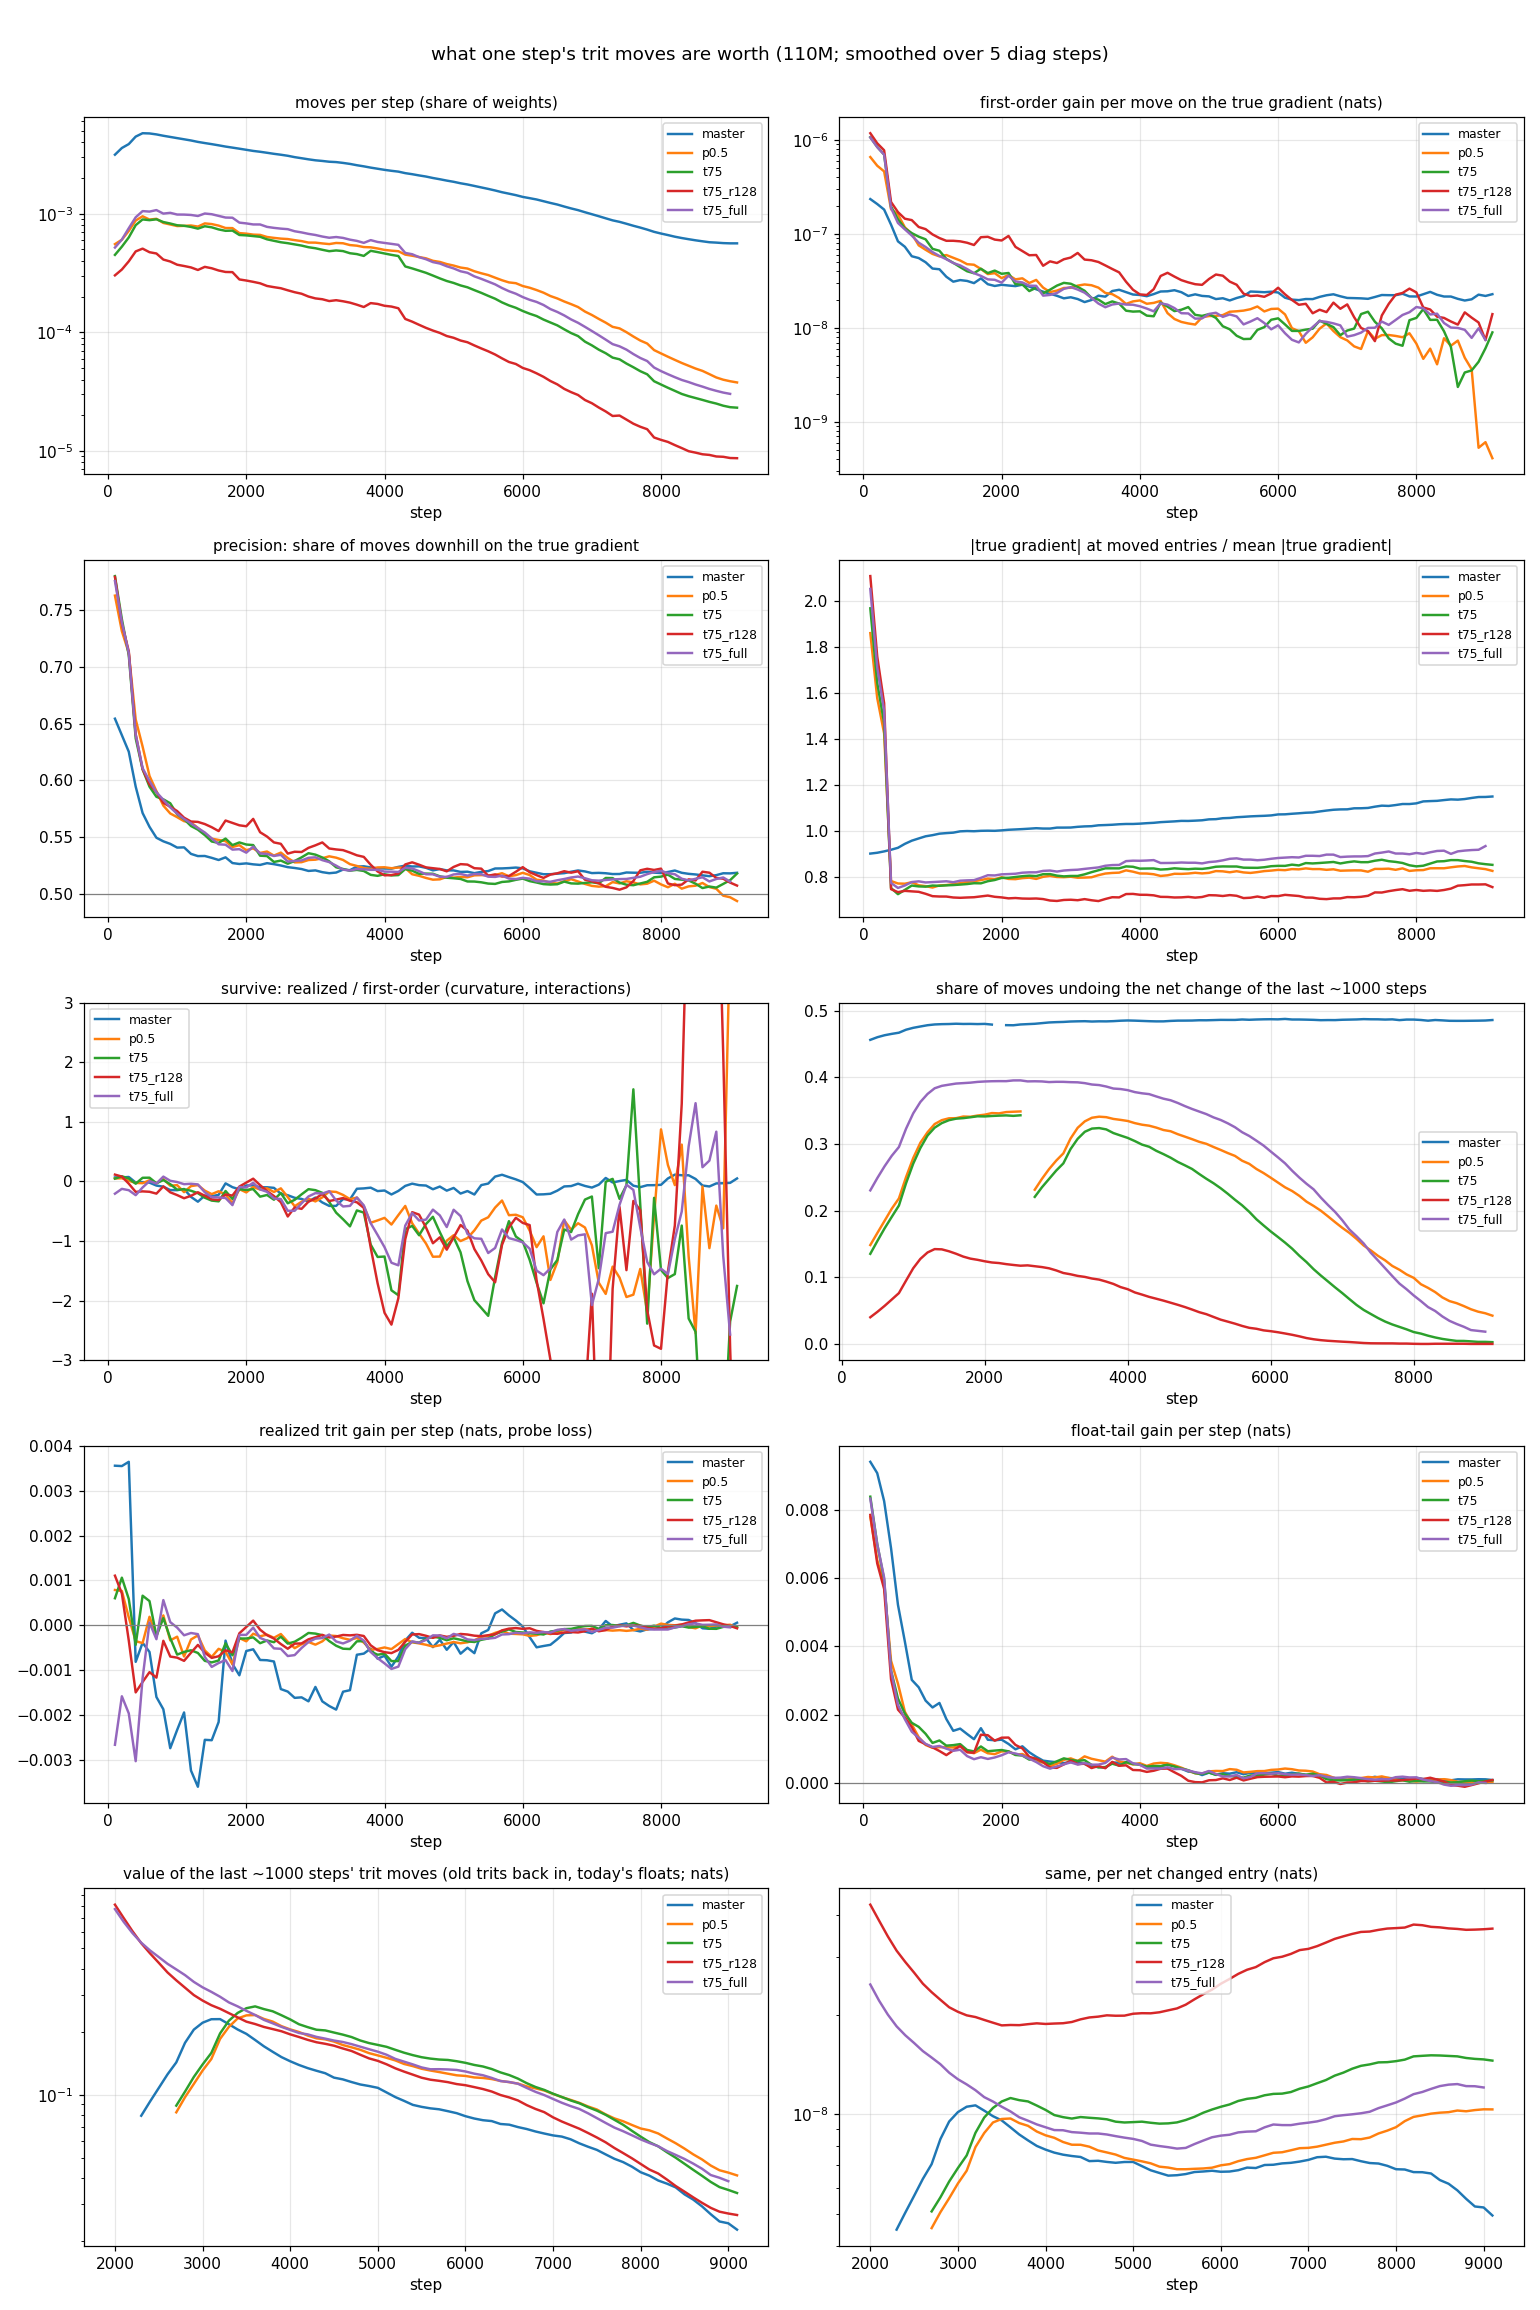
\includegraphics[width=\columnwidth]{figures/movediag.png}
\caption{Move diagnostics against training step, master and TTF ($p=0.5$; $p=0.75$ + annealed leak at ranks 128, 512 and
full): moves per step, first-order
gain per move, precision, gradient size at moved entries, undo share, the float tail's gain, and the value of the last
1000 steps of moves (total and per changed entry).}
\label{fig:movediag}
\end{figure}

\subsection{Budget frontier}
We trained TTF to budgets of 1000--9155 steps, each with its own cosine (Table~\ref{tab:frontier}). TTF trails
master at 1000 steps and leads from 4000 steps on, with $p=0.5$ already from 2000.

\begin{table}[t]
\caption{TTF minus master at each training budget (110M, rank 512, each budget with its own cosine).}
\label{tab:frontier}
\resizebox{\linewidth}{!}{\begin{tabular}{lrrrrr}
\toprule
steps & 1000 & 2000 & 4000 & 6000 & 9155 \\
\midrule
$p=0.5$ & $+0.029$ & $-0.014$ & $-0.035$ & $-0.047$ & $-0.043$ \\
$p=0.75$ + annealed leak & $+0.016$ & $+0.005$ & $-0.028$ & $-0.038$ & $-0.042$ \\
\bottomrule
\end{tabular}}
\end{table}

\section{How ternary networks trained from scratch differ from full precision}\label{sec:organise}
A ternary model trained from scratch finds its own solution. We compared it with full precision at 110M parameters
with the same architecture, data and token budget (Wikipedia, 300M tokens): the full-precision model and a second
full-precision seed against TTF from scratch with two seeds. Raw weights cannot be compared: hidden units can be
permuted, and with the norm gains folded in the residual stream can be rotated, without changing the function, and trit
agreement is at chance even between the two TTF seeds (0.350 against 0.350). We therefore compare representations and
statistics that do not depend on the basis.

\begin{table}[t]
\centering
\caption{Full precision against ternary from scratch at 110M (blocks 1 $\to$ 11 for the residual stream; weights averaged
over layers). CKA: linear centred kernel alignment of the residual stream on 16 Wikipedia windows
\citep{kornblith2019similarity}; two untrained networks of this architecture reach 0.880 on the same windows (see text).}
\label{tab:organise}
\resizebox{\linewidth}{!}{\begin{tabular}{lrr}
\toprule
 & full precision & TTF from scratch \\
\midrule
residual norm & 265 $\to$ 678 & 55 $\to$ 265 \\
largest / median dimension (rms) & 40 $\to$ 12 & 8.5 $\to$ 10 \\
excess kurtosis across dimensions & 216 $\to$ 38 & 15 $\to$ 18 \\
effective rank, value / output projections (fraction of full) & 0.26 / 0.28 & 0.46 / 0.46 \\
effective rank, gate / up projections & 0.34 / 0.39 & 0.55 / 0.58 \\
log-log singular value slope & $-0.50$ & $-0.33$ \\
zero trits (GPTQ of full precision / TTF) & 42\%, by input channel & 23\%, spread evenly \\
residual CKA between two seeds & 0.816 & 0.890 \\
\bottomrule
\end{tabular}}
\end{table}

\paragraph{Organisation.} The two families differ in a consistent way (Table~\ref{tab:organise}). The full-precision
model writes a large, nearly constant offset into two residual dimensions: at block 1 the top four dimensions hold 76\%
of $|h|^2$, and 96\% of that is the same on every token. These are the massive activations of \citet{sun2024massive},
which act as fixed biases. Ternary training from scratch never builds the offset. It spreads the signal over many coarse
weights instead: higher effective rank, flatter spectra, and zeros spread evenly over the inputs. Two ternary seeds are
also more alike than two full-precision seeds (residual CKA 0.890 against 0.816), and full precision against ternary is
below both (0.66--0.73). Linear CKA has no zero point for unrelated networks on the same text. On the same windows two
untrained networks of this architecture already reach 0.880, a trained full-precision model against an untrained one
0.08, a fixed random embedding of the current token alone 0.22, and the full-precision seeds with their token pairing
permuted 0.00 (the debiased estimator of \citet{song2012feature} gives the same values). The seed-to-seed values
therefore do not by themselves show shared learned features; what the comparison supports is that full precision
against ternary (0.70) sits below both families' seed baselines, well above the token-identity level.
With the final recipe (rank 512, $p=0.75$, annealed leak; two new seeds) the TTF seeds reach 0.888, TTF against an
untrained network 0.07--0.08, and TTF against the current-token embedding 0.16--0.19 (full precision 0.22--0.24); full
precision against these seeds is 0.66--0.73.

\paragraph{Basins.} The straight path in weight space \citep{frankle2020linear} from the full-precision model to the ternary model trained from
scratch rises to a loss of 8.45, as between two full-precision seeds (9.6): the two are separate basins. Basins are kept
whatever the precision. A full-precision network trained for 50M tokens from the dense weights of the ternary model
stays in the ternary model's basin (one-to-one neuron correlation 0.90, CKA 0.98 with it; CKA 0.78 with full precision)
and still reaches 2.721 against full precision's 2.716 on the same windows. At this size the two families are equally
good basins for both precisions; the precision does not choose the basin.

\paragraph{Sharpness.} Ternary minima are not flatter. Under relative Gaussian noise on the effective weights of every
linear the two ternary seeds lose more than the two full-precision seeds (loss rise at noise 0.3: $+0.140$ / $+0.150$
against $+0.100$ / $+0.102$), and the top Hessian eigenvalue of the linears, scaled by $|W|^2$ to be invariant to
rescaling, is about twice as large ($2.1$--$2.6\times10^6$ against $1.0$--$1.2\times10^6$). Along the lattice the two
families lose about the same: moving a random 1\% of every linear's weights by one grid step costs $+0.016$ / $+0.020$
for TTF and $+0.019$ / $+0.016$ for full precision (one step of its own ternary rounding). The companion paper uses these
measurements to ask what a conversion of a pretrained full-precision model inherits.

\section{Float-free ternary models}\label{sec:floatfree}
TTF's lead could come from the float extras it trains beside the trits. At 110M a quarter of the parameters are float
(Table~\ref{tab:floats}), mostly the embedding. We remove the float extras and then make the embedding ternary too: $E_{ij}=s_0\,r_ic_j\,T_{ij}$ with trits $T$, learned row and column scales and
a fixed base scale, tied to the output head, its trits trained by TTF from the sum of the lookup and head gradients
(for master, an absmean latent with the STE). Only scales and norm gains stay float.
\begin{table*}[t]
\centering
\caption{Float-free variants (110M, rank 512, final recipe; fixed windows). Master with all float extras is the
two-seed mean, without extras the three-seed mean.}
\label{tab:floatfree}
\resizebox{\linewidth}{!}{\begin{tabular}{lrrrr}
\toprule
 & \multicolumn{2}{c}{TTF} & \multicolumn{2}{c}{master} \\
 & Wikipedia & FineWeb-Edu & Wikipedia & FineWeb-Edu \\
\midrule
all float extras (reference) & 2.6728 & 3.6226 & 2.7166 & 3.6830 \\
no extras (no $PQ^\top$, no row / column scales) & 2.6907 & 3.6435 & 2.736 & 3.707 \\
row / column scales only & 2.6794 & 3.6309 & 2.7209 & 3.6904 \\
\quad + ternary tied embedding (only scales float) & 2.8106 & 3.7758 & 2.9312 & 3.9492 \\
\quad + ternary untied embedding and head & 2.8273 & 3.8100 & & \\
float extras, tied ternary embedding $20\times$ wide + ternary projection & 2.7265 & 3.6832 & & \\
\quad + ternary adapters of rank 320 (all-ternary) & 2.7343 & 3.6885 & & \\
\bottomrule
\end{tabular}}
\end{table*}

\paragraph{Without the extras.} TTF with no float extras (no $PQ^\top$ and no row or column scales, so each layer's
output scale is the fixed $\beta$) ends at 2.6907 on Wikipedia. That is 0.018 behind TTF with the extras, but 0.045
ahead of plain master and 0.026 ahead of master \emph{with} the extras (0.064 and 0.040 on FineWeb-Edu). The extras are
worth about 0.02 to either method, and TTF's lead does not come from them. Row and column scales alone recover two
thirds of it, and the rank-16 float adapter adds the remaining 0.007.

\paragraph{Ternary embedding and head.} With an untied ternary embedding and output head (49.2M ternary embedding
weights with row and column scales, and 134M parameters, of which 0.2M are float besides the norm gains), TTF ends 0.148
behind the same model with a float embedding. The whole model then packs into 27 MB, against 66 MB with a 16-bit
embedding, which is 2.5 times smaller for 0.15 nats. Tied, the ternary embedding does slightly better with half the
embedding weights (110M parameters, 22 MB packed). Master with the same tied ternary embedding, an absmean latent with
the straight-through gradient, falls further behind. Without float embeddings TTF's lead grows from 0.044 to 0.121 on
Wikipedia and from 0.060 to 0.173 on FineWeb-Edu. With the same row and column scales and nothing else, TTF leads master
by 0.042 (0.060 on FineWeb-Edu).

A ternary embedding with the bytes of a float one does better again. Packed trits cost 1.6 bits against fp32's 32, so
a table 20 times as wide ($32000\times15360$ trits, the same 98 MB) followed by a ternary projection to the model width
fits in the same memory. Both are trained by TTF, and their product, formed once per step, is also the tied head. This
model goes 61\% of the way from the same-width ternary embedding to the float one, and it is level with master with a
float embedding on FineWeb-Edu (0.010 behind on Wikipedia). Turning the rank-16 float adapters into ternary factors at
fp32's bytes as well (rank 320, trained by TTF, with the row scales of one factor starting at zero) costs little more.
In this all-ternary model only the per-row and per-column scales and the norm gains stay float, and it is level with
master's float-embedding model on FineWeb-Edu and 0.018 behind it on Wikipedia.

\paragraph{Integer embedding and head without a dense matrix.} The ternary embedding gives up 0.14 nats, and $k$-level codes
recover most of it at a few bits. Each row is split into groups of 64 with a learned offset and step,
$W_{ij}=\ell_{ig}+s_{ig}\,q_{ij}$, $q_{ij}\in\{0,\dots,2^b-1\}$. TTF moves a code by one level when its accumulator entry
reaches $\theta$, and $\ell,s$ train in the float tail. Vocabulary-sized matrices make a dense update path expensive:
at 27B a bf16 copy of the head, its fp32 gradient sum and the codes take about 18 GB. The factored update never forms
either. The head loss runs over token chunks with logits from codes dequantized in vocabulary chunks, and keeps the
micro-batch's $\partial L/\partial z$ (bf16) and the head input as the gradient's factors. The embedding's gradient is
the distinct looked-up rows with their summed $\partial L/\partial h$. A tied matrix adds both factor sets in one
update, and the accumulator's $U$ is stored per chunk of 8192 rows. The factors give $\partial L/\partial W$, but the
code moves along $\partial L/\partial q=s\,\partial L/\partial W$. A step that is constant along a row cancels in the
row-normalised update, so only its variation within the row is applied. A code fires on $\rho A\ge\theta$ with
$\rho=s/\mathrm{rms}_{\text{row}}(s)$, moves by $\mathrm{sign}(\rho A)$ and spends $\theta/\rho$ of $A$. The sign matters.
After training, 56--78\% of the group steps are negative (a group can flip its order), and using $|s|$ moves those codes
the wrong way, which at 15M (300 steps, tied 4-bit) costs 0.15 nats. With the signed ratio, the factored update matches
the dense one (5.706 against 5.709, the mean of two seeds, with a float embedding at 5.622). Peak memory is unchanged at 15M (1.20 vs
1.18 GiB). On Qwen3.5-0.8B (2-bit embedding, 3-bit head) it is 5.4 GiB, where the dense path needs 9.0 GiB at the
first step and then runs out of memory under an 11 GiB cap. At 27B it frees about 8 GB on the head's pipeline stage.

\subsection{Ternary adapters on converted networks}\label{sec:tadapt1}
The ternary factors above are a general tool. Any low-rank correction $U(Dx)$ with $D$ and $U$ ternary (each with row
and column scales) is just two more ternary layers, and TTF trains them with the same accumulator, threshold and step
scale as the main weights. The companion paper on conversion uses them to hold what rounding a pretrained model
removes (fitted to the residual in the layer's output metric, the objective QERA \citep{zhang2025qera} solves in closed
form for float low-rank terms, then trained). Two observations belong here, because
they are about TTF itself. First, TTF trains the extra trits rather than merely storing them. On Qwen3.5-0.8B,
adapters of rank $0.1\times\min(K,N)$ (13\% more trits) after 1000 TTF steps beat the plain ternary model after 3000
(Wikipedia 2.9988 against 3.0087, chat 2.8344 against 3.0633). Second, the adapter trits are where TTF moves first. From
the converted state with every float frozen, 100 steps at $\theta=16$ change 2.47\% of the adapter trits and 0.18\% of
the main ones, and by step 90 the loss has fallen from 3.4372 to 3.1060 (eight fixed Wikipedia windows) through trit
moves alone.

\section{Memory and speed}\label{sec:memory}
\paragraph{Budget.} Per weight TTF stores the trit (0.2 bytes packed) and, amortised, the factored second moment and the
rank-$r$ factors (Table~\ref{tab:state}). With a 12-bit accumulator the 2.9B model at rank 1536 keeps about 1.18 bytes
of optimizer state per weight, against 12 for master. At the 23.0B shape, rank 1024 costs 0.50 bytes per weight (0.33
numbers). The rank fit of Section~\ref{sec:rank} puts that rank 0.061 above full rank there (0.060 to 0.063 over $g$'s
95\% range, or 0.082 for a fixed cost per halving). By the share reading, 0.33 numbers per weight is half the
break-even state, where the line through the 1.3B and 2.9B points has TTF about 0.03 behind master (an extrapolation
over a factor of 2.5 in width). A budget model predicts every measured point within 0.4 GiB.

\begin{table*}[t]
\centering
\caption{One optimizer step of Qwen3.5-0.8B, profiled (16 micro-batches of 2048 tokens, RTX 4070 with a Ryzen 3950X,
before the speed changes listed in the text). Seconds per step; peak allocated memory in GiB. The conversion runs
distil from the full-precision teacher with the head frozen; the bf16 AdamW reference uses cross-entropy only.}
\label{tab:profile}
\resizebox{\linewidth}{!}{\begin{tabular}{lrrrr}
\toprule
 & TTF from scratch & conversion, ternary adapters & conversion, no adapters & bf16 AdamW \\
\midrule
wall time & 9.46 & 23.37 & & \\
GPU kernels & 9.00 & 17.25 & 12.84 & 9.11 \\
\quad head and loss & 2.47 & 4.01 & 4.01 & 2.47 \\
\quad activation recompute & 1.11 & 1.99 & 1.34 & 1.35 \\
\quad teacher & & 1.75 & 1.75 & \\
\quad main TTF update & 1.40 & 1.37 & 1.38 & \\
\quad adapters (forward and backward + TTF) & & 1.93 + 1.75 & & \\
peak memory & 5.42 & 8.22 & 8.16 & 7.62 \\
\bottomrule
\end{tabular}}
\end{table*}

\paragraph{Where a step's time goes.} We profiled one optimizer step of Qwen3.5-0.8B, with every GPU kernel and CPU op
attributed to the innermost named range (Table~\ref{tab:profile}). Trained from scratch (embedding and head trainable,
8-bit-moment float optimizer, no distillation), TTF is GPU-bound, and the 248k-vocabulary head and loss take 27\% of the
GPU time. TTF's per-micro-batch update is 0.36~s of GPU but 3.3~s of CPU in small elementwise operations. The fused
micro-batch kernel removes that CPU time (four Triton kernels instead of about fifty operations). At the peak, inside
the backward pass, 3.09~GiB persist from the start of the step (float gradients 0.95, embedding 0.95, float optimizer
0.48, TTF factors 0.61, trits 0.09). The step has allocated another 3.64~GiB by then and freed 1.33~GiB of the
persistent blocks, which gives 5.42~GiB.

The full-precision reference keeps all parameters in bf16 and uses fused AdamW on the same model, data and machine.
With the teacher it does not fit in 12~GB, so it trains on cross-entropy only. Its kernels take 9.11~s per step against
TTF's 9.00~s, and its peak memory is 7.62~GiB (gradients 1.40, AdamW moments 2.80, parameters 1.40) against TTF's 5.42.
A TTF step costs what an AdamW step costs, with 29\% less memory and without an fp32 master copy (which the bf16
reference also omits). In conversion recovery with ternary adapters, the head and loss, the activation recompute, the
adapters, the teacher and the two TTF updates share the time (the linear attention takes another 1.5~s). Without
adapters, the head and loss take 31\% of the kernel time, the teacher 14\% and the recompute 10\%.

Three later changes took the adapter recovery step from 24.90 to 16.99~s on an RTX 4070. The update fires without
a host synchronisation per layer, the per-micro-batch update is fused into four Triton kernels, and a frozen head's
loss and input gradient are computed in one pass, without recomputing the 248k-wide logits. Each stays within the run-to-run noise of
losses and trits. Two further changes are now defaults. The input gradient is computed in one int8 slice per row (7
bits, on the int8 tensor cores, where two slices were as accurate as bf16), and TTF's fp32 products use TF32, with the
orthonormalisation kept in full fp32. Over 1000 steps of Qwen3.5-0.8B recovery each is level with the reference. With
one slice, Wikipedia, chat and mix differ by $+0.0003$, $+0.0002$ and $+0.0023$, and the paired train-loss gap stays
between $-0.003$ and $+0.007$. One slice takes the step of a 27B slice from 5.77 to 5.27~s on a laptop RTX 4080.

\paragraph{Measured.} A 23.0B-parameter model (22.85B ternary) trains on one 16 GB RTX 4070 Ti Super. It uses 11.1 GiB of
GPU memory at ranks 256 and 512 with the state offloaded to the host (11.2 and 17.0 GiB there), and 11.6 GiB at rank
1024 with the 12-bit accumulator. Host offload with asynchronous copies costs no time at 1.3B (2.80 against 2.79 s per
step). We trained it for 500 steps of one 2048-token sequence (1M tokens, rank 1024, the 12-bit accumulator and 70\% of the
state on the GPU) under a 22.4 GiB cap on an A100, which is a 24 GB card's usable memory. It peaks at 17.3 GiB and runs
at 38.5~s per step, and the validation loss falls from 11.33 at initialisation to 6.40. This is a result about memory
and stability, not a converged model, since 1M tokens are far from enough for 23.0B parameters. At its leanest (rank
256, all state in host memory, one 2048-token sequence per step, the loss in 256-token chunks, activations recomputed
per block) the same model peaks at 9.73 GiB allocated (10.8 GiB by nvidia-smi) on an RTX 3090 Ti and runs at 19.5~s per
step. The trits take 4.26 GiB, the float tail with its gradients and optimizer 1.46 GiB, and TTF's state 2.69 GiB on
the host.

Qwen3.8-27B, converted by streaming GPTQ \citep{frantar2023gptq} in 20 minutes on the same card (output-space error 0.051
against 0.167 for nearest rounding), carries a float 248k-vocabulary embedding and head (4.7 GiB in bf16). With all of
TTF's state on the GPU (rank 256, 2.46 GiB) and 16 micro-batches of one sequence per step, it trains under the 22.4 GiB
cap. It peaks at 21.2 GiB (trits 4.53, float tail 5.0, 12.6 GiB allocated between steps) and takes 211~s per 32k-token
step with the trits frozen and 235~s once they move. On the first eight Wikipedia windows of 2048 tokens, the
full-precision model scores 1.9034, the model right after the streaming conversion 3.8507, and the model after 60
recovery steps (about 2M tokens) 2.3644, so 76\% of the conversion's loss is recovered. Packed this way, the model also
runs inference on a 12 GB laptop GPU (RTX 4080 Laptop, 9.1 GiB peak, the embedding read from pinned host memory) at
22.7 tokens/s, with the trits in a 2-bit layout and an int8 $\times$ trit GEMV. Step time and peak memory against rank
at 110M and 340M are in Section~\ref{sec:rank}. At 1.3B, batch 16 does not fit in 16 GB for either method.

\paragraph{27B on two GPUs.} Qwen3.8-27B, converted with ternary adapters of rank $0.2\min(K,N)$ (the companion
paper) and with int-$k$ embedding and head codes, trains pipeline-parallel over two 96 GB RTX PRO 6000 GPUs (one stage
each, 1F1B over 16 micro-batches of 2048 tokens, TTF rank 1536) at 27.0~s per 32k-token step, peaking at 72.8 and
66.5~GiB with the last 15 blocks of each stage keeping their activations. The first stage holds more micro-batches in
flight, so a kept block costs it about twice as much (2.3 against 1.2~GiB). Per stage and step, profiled before the
change below, TTF's update takes
10.9~s (the orthonormalisation 4.7~s over 185 calls, the per-micro-batch accumulation 2.4~s, firing 0.35~s), the
ternary forward 5.7~s and the input gradient 4.3~s, the second stage's head and distillation loss 1.4~s, and each
stage waits 6--9~s for the other. The second stage's last micro-batch ends with its per-layer updates (the step's basis
turn, firing and spend). Running them after its input gradient is sent rather than before (the same updates, later)
removes most of the first stage's wait and takes the step from 32.8 to 27.0~s. On one GPU the rank costs time (47.5,
54.3 and 59.8~s per step at ranks 1024, 1536 and 2048), while keeping more blocks' activations instead of recomputing
them saves almost nothing (within 1~s from 1 to 13 blocks kept). Data parallelism does not help here, because each rank
repeats the whole update.

\paragraph{Micro-batches without a dense gradient.} When a batch does not fit in one pass it is split into $M$
micro-batches. Gradient accumulation would keep a dense $N\times K$ sum per layer, as large as the model, which is the
memory TTF removes. Instead each micro-batch's gradient enters the state and is discarded. The momentum steps once per
micro-batch (decay $\beta_1^{1/M}$), the batch's second moment is assembled from the micro-batches' squares plus their
cross terms through a random sketch, and the accumulator, firing and spend run once per step
(Appendix~\ref{app:micro}). At 110M, $4\times4$ micro-batches match one pass of batch 16 after 1000 steps (3.6078
against 3.6126 on the 974 fixed windows) with 1.65 instead of 3.75 GiB and 4\% more time, and the step agrees with the
dense batch path to a cosine of 0.996--0.999. A 10B model with batch $16\times2048$ then fits a 40 GB A100 (18.3 GiB, 55.7 s per step)
instead of needing 41.9 GiB in one pass. Without momentum (the final recipe) each micro-batch enters the accumulator
directly, normalised by the previous step's $v$ mixed with its own squares. Over the full 9155-step schedule at 110M,
$4\times4$ micro-batches end at 2.6733 against 2.6728 for one pass of batch 16, with 3.1 instead of 7.4 GiB.

\paragraph{Storage formats.} The accumulator needs about 12 bits. With 7, 5, 4 and 3 mantissa bits the loss changes by
$+0.0005$, $+0.0018$, $+0.052$ and $+0.149$, and a real 12-bit store matches the simulation (2.7082 against 2.7087). An
int8 accumulator costs 0.01--0.02, because rounding noise integrates over the accumulator's memory.

\paragraph{Multi-GPU training.} We built and used both data and pipeline parallelism. In \emph{data parallel} training
every rank holds the whole model and draws its own micro-batches. Before a layer's update its gradient is averaged
across ranks with one all-reduce per layer, as for master. With the factored update the factors $(g_y, x)$ are reduced
instead of the dense $N\times K$ gradient, about $(N+K)(k+2r)$ floats per layer and micro-batch. Every rank then runs
the same update and moves the same trits, and trits are never sent. Two processes on one GPU, and two machines over
gigabit Ethernet (two RTX 4070 Ti Super, NCCL over sockets), keep the packed trits bitwise identical at every check
(steps 0, 100 and 200). The two machines ran at 18~s per step against 28~s on one, and after 300 steps their validation
loss was within 0.03 of the single-GPU run, which draws different batches. On Qwen3.8-27B, two RTX 4090 without
peer-to-peer access take 27.8~s per 32k-token step against 61.8~s on one RTX 3090 Ti. Rank 0's losses match the
single-GPU run (0.734 and 0.889 against 0.736 and 0.890 at steps 1350 and 1360), the run stops and resumes, the trits
agree on both ranks at step 1400, and each rank peaks at 19.7 GiB. Four RTX 4090 on two NUMA nodes without peer-to-peer
access take 18.7~s, bound by communication. The distillation cache is read rank-aware, so the ranks see disjoint
teacher shards. In \emph{pipeline parallel} training each stage owns a contiguous block of decoder layers (the embedding on the first stage, the
final norm and head on the last), holds and updates only those layers' trits and TTF state, and only hidden states and
their gradients cross stages. Stage checkpoints merge into a single-GPU checkpoint. On a two-stage test model the
evaluation forward is identical, ten training steps agree to about $10^{-5}$ (the float tail's stochastic rounding is
per process), and the merged checkpoint resumes on one GPU to the same evaluation. The 27B continuation on four RTX
4090 in four stages ran at 19.0~s per step with losses identical to the single-GPU run at step 1360, for 1000 steps on
its mixture. Tensor parallelism, which would split the accumulator's factors with the layer ($U$ by rows, $V$ by
columns, with a reduction of $\tilde A^\top U$ across row shards in every subspace-iteration step), is not built.

\section{Related work}\label{sec:related}

\paragraph{Ternary and binary networks with latent weights.} BinaryConnect \citep{courbariaux2015binaryconnect} and the
straight-through estimator \citep{bengio2013estimating} established latent-weight training of quantised networks. BitNet
b1.58 \citep{ma2024era} and Spectra/TriLM \citep{kaushal2025spectra} scale it to ternary LLMs and are our master
reference.

\paragraph{Converting pretrained models to ternary.} The Hugging Face recipe \citep{mekkouri2024bitnet} fine-tunes
Llama-3-8B to ternary weights with a warmup that phases the quantisation in. \citet{nielsen2025continual} find that
switching from 16-bit to 1.58-bit pretraining beats ternary training from scratch, and that phasing in and keeping the
optimizer state soften the loss spike, though further training removes the difference. BitNet Distillation
\citep{wu2025bitdistill} adds normalisation before the output and down projections, continues pretraining and distils
logits and attention relations, for task-specific Qwen3 models up to 4B. It observes that continued pretraining moves the
weight distribution towards that of ternary models trained from scratch. Post-training ternarisation \citep{wang2026ayot}
calibrates reasoning models on their own reasoning traces, and LLM-QAT \citep{liu2024llmqat} trains quantised models on
text sampled from the model itself. All of these keep latent weights or use no training. A companion paper converts
pretrained models with TTF, training the trits with its sublinear state. Low-rank terms that reconstruct the
quantisation error were first chosen heuristically, and QERA \citep{zhang2025qera} derives them in closed form for the
layer's output error rather than its weight error. They are float terms on a fixed quantised base, whereas the
companion paper's adapters are ternary and trained with the base.

\paragraph{Training without a full-precision master copy.} Bop \citep{helwegen2019latent} flips binary weights when a
per-weight gradient EMA crosses a threshold. It keeps one float per weight and one timescale. DQT \citep{zhao2025dqt}
updates low-bit weights directly with stochastic rounding but keeps per-weight optimizer moments (AdamW in its main
experiments). ECO \citep{nikdan2026eco}
feeds the quantisation error back into the optimizer's momentum. Q-GaLore \citep{zhang2024qgalore} keeps INT8 weights
updated by stochastic rounding with low-rank projected Adam. Per weight, TTF keeps only the ternary value, and all of its
optimizer state is sublinear.

\paragraph{Low-rank and factored optimizer state.} Adafactor \citep{shazeer2018adafactor} factors the second moment as
we do. GaLore \citep{zhao2024galore} projects gradients to a low-rank subspace and runs Adam there. MoFaSGD
\citep{mahdavinia2025mofasgd} keeps a dynamically updated low-rank SVD of the momentum, and ReLoRA
\citep{lialin2023relora} restricts updates to low rank and merges them periodically. All keep full-precision weights.
TTF's spent moves land in full-rank discrete weights, so the cumulative change is not rank limited.

\paragraph{Fine-tuning ternary models.} Low-rank ternary adaptation \citep{manolache2026ternary} fine-tunes trained
ternary models with a multiplicative ternary adapter (keep, zero or flip the sign of each weight) built as a Kronecker
product of ternary factors, so a zero weight cannot be reactivated. We train from scratch, and a move may go to or from 0.

\paragraph{Learning-rate schedules.} Warmup-stable-decay \citep{hu2024minicpm,hagele2024scaling} and re-warming for
continued pretraining \citep{gupta2023continual,ibrahim2024simple} (Section~\ref{sec:results}).

\paragraph{Compressed optimizer state.} 8-bit \citep{dettmers2022optimizers} and 4-bit \citep{li2023memory} Adam
quantise the moments block-wise. MicroAdam \citep{modoranu2024microadam} keeps a compressed gradient window with error
feedback, and Adam-mini \citep{zhang2025adammini} shares one second moment per parameter block. All shrink the bytes per
number but keep a full-precision weight beside them. TTF's accumulator tolerates 12 bits (Section~\ref{sec:memory}), so
these quantisers compose with it. What TTF removes is the weight copy and the per-weight count of state numbers.

\paragraph{Sign-based updates.} signSGD \citep{bernstein2018signsgd} and Lion \citep{chen2023lion} move every weight by
a fixed amount in the sign of a (momentum) estimate at every step. A TTF move is also a fixed-size sign step, but it is
taken only when the integrated evidence crosses the threshold, and that evidence is then spent, and between moves nothing
changes. Bop \citep{helwegen2019latent} is the binary analogue with one float per weight, and OvSW \citep{xiang2024ovsw}
reports that over half of a latent-weight binary network's signs never change in training. TTF shows the same inertia,
set by the state. In early 340M runs 23\% of the trits never moved at rank 512, 33\% at rank 256 and 52\% at rank 128
(16\% with the $p=0.5$ schedule at rank 512).

\section{Discussion}\label{sec:discussion}
\paragraph{From memory-bound to compute-bound.} With master weights, the size of model one can train or adapt is set by
memory. Master needs twelve bytes of optimizer state per weight on top of the weights, gradients and activations. With TTF the state
is at most about one byte per weight (half a byte for the 23B model at rank 1024) and the weights are 0.2 bytes, so a 23B model fits a 16 GB card and a 27B model recovers
on a 24 GB card (Section~\ref{sec:memory}). What remains binding is arithmetic. The 23.0B model trains at about 105
tokens per second on one RTX 3090 Ti and Qwen3.8-27B recovers at about 140. A billion tokens would take months on
one card, while ten million, the scale of a fine-tune, take about a day. The question for a given budget therefore
moves from whether a model fits to how many tokens one can afford.

\paragraph{Kernels and hardware.} Our training kernels hold trits packed and multiply them on int8 tensor cores, and
inference uses a 2-bit layout with four-way 8-bit dot products (22.7 tokens per second for the 27B model on a laptop GPU).
Neither exploits that a ternary product is an addition or a sign change. Since TTF leaves no full-precision weight in
the training loop, the forward and backward products are a large share of its cost (we have not profiled the
split), and kernels and hardware built for ternary
operands are where further speed would come from, but we have not built them.

\paragraph{Who can train and adapt large models.} Training and fine-tuning tens of billions of parameters has needed
clusters of data-centre accelerators. TTF moves it onto a single consumer card, within reach of university groups,
small companies and individuals, for training from scratch at modest scale and, more realistically, for converting and
adapting existing open models.

\paragraph{Misuse.} The same lowering of the barrier applies to people who would adapt models to harmful ends, such as removing
a model's safety training, specialising it for malware, fraud or disinformation, or training a misaligned model with no
oversight. Fine-tuning, which needs few tokens, is the relevant case, and it is exactly where a single card now
suffices. Safety measures that rely on the cost of training, such as thresholds on compute or on access to large
accelerators, become weaker as that cost falls, which puts more weight on safeguards that hold after release, such as
alignment that resists further training, and on how open weights are released. We release the method and its code
because master-free training already exists at higher cost and its benefits are broad, but we note the risk so that it
is weighed rather than assumed away.

\begin{table*}[t]
\centering
\caption{Zero-shot accuracy (2.9B: FineWeb-Edu; 1.3B: Wikipedia; 300M tokens each). HellaSwag and ARC-Challenge
acc\_norm. Standard errors 0.004--0.014. 1.3B: two seeds each; its master is master + extras (lr 5e-4).}
\label{tab:zeroshot}
\begin{tabular}{lrrrrr}
\toprule
 & \multicolumn{3}{c}{2.9B} & \multicolumn{2}{c}{1.3B} \\
task & TTF 1536 & TTF 1024 & master & TTF 1024 & master \\
\midrule
LAMBADA & 0.193 & 0.195 & 0.183 & 0.160, 0.155 & 0.152, 0.138 \\
HellaSwag & 0.291 & 0.290 & 0.288 & 0.272, 0.272 & 0.269, 0.269 \\
PIQA & 0.600 & 0.597 & 0.598 & 0.547, 0.550 & 0.532, 0.550 \\
ARC-Easy & 0.470 & 0.453 & 0.453 & 0.336, 0.330 & 0.339, 0.339 \\
ARC-Challenge & 0.243 & 0.249 & 0.222 & 0.224, 0.228 & 0.216, 0.212 \\
WinoGrande & 0.496 & 0.511 & 0.501 & 0.499, 0.531 & 0.509, 0.504 \\
\bottomrule
\end{tabular}
\end{table*}

\section{Limitations}\label{sec:limits}
\begin{itemize}
\item \textbf{Scale and tokens.} The largest comparison is 2.9B at 300M tokens, and the 110M lead was tested to 600M
  tokens. Budgets are far below compute-optimal for 340M and above. The gap's independence of training length
  (Table~\ref{tab:depth15}) is measured at 15M only, up to five times compute-optimal, one run per point.
\item \textbf{Seeds.} Two to three seeds at 110M and 340M, two at 1.3B (rank 1024 and master, where TTF's seeds differ
  by 0.009 on Wikipedia and 0.012 on FineWeb-Edu, more than master's 0.001 and 0.003), and one at 2.9B and for the other
  1.3B ranks.
\item \textbf{Master tuning at 2.9B.} Two learning rates (4e-4 better than 2.5e-4), and a better master would move the
  2.9B points of Section~\ref{sec:rank}.
\item \textbf{Mixed data across sizes.} 1.3B is on Wikipedia, 2.9B on FineWeb-Edu, and the curve of Section~\ref{sec:rank}
  uses each size's training distribution.
\item \textbf{Output projections.} The accumulator's orthonormal basis $V$ sits on the input side of every layer. In
  converted models we later found that the layers reading the MLP hidden state or the attention output (the MLP down
  projection and the attention output projections) moved almost no trits at ranks 64 to 512, because the persistent part
  of their gradient lies on the output side. The from-scratch runs reported here do not show this. In the 110M runs of
  Table~\ref{tab:rank110}, by the last step the down projection had moved 63\%, 85\%, 88\% and 89\% of its trits at
  least once (ranks 128, 384, 512 and full, the 512 figures from that rank's second seed), against 63\%, 84\%, 86\% and 87\% of all trits. The attention output
  projection had moved 63\%, 81\%, 83\% and 83\%, more than the value projection (54\% to 77\%). Over the last fifth of
  training the down projection moved trits at 0.87 to 1.06 times the mean rate of the five other types and the output
  projection at 0.70 to 0.87 times, again above the value projection. We ran a basis on the output side of the down
  projections once, at 110M for 2000 steps against the same run with the input-side basis (same seed and data). Its
  fixed-window Wikipedia loss was lower by $0.0065 \pm 0.0008$ (paired over windows, 63\% of windows better), and the
  down projections' moved share rose only from 0.69 to 0.70. One run does not measure the run-to-run spread, the full
  schedule is untested, and the option is not in the released code.
\item \textbf{Micro-batches.} The micro-batch update without momentum (Appendix~\ref{app:micro}) was run for the full
  schedule at 110M only, and memory and speed at 10B were measured with the short-momentum version.
\item \textbf{Downstream evaluation.} Zero-shot tasks are near chance at these sizes (Table~\ref{tab:zeroshot}). At 2.9B
  TTF is level with master within one to two standard errors, and the tasks cannot separate the methods at this
  budget. At 1.3B the two are also level, with LAMBADA slightly ahead for TTF in both seeds.
\end{itemize}

\section{Open directions}\label{sec:open}
Several directions are built only in part or not at all. The mechanisms we tried are listed with their results in
Appendices~\ref{app:history} and~\ref{app:variants}.

\paragraph{Mixture of experts.} With one accumulator per ternary expert, the experts give TTF the gain they give master
(at rank 320 and a third of the training, fixed windows on Wikipedia: TTF from 3.0531 dense to 2.9901 with 8 experts of
hidden 1024 and top-2 routing, master + extras from 3.0434 to 2.9780), and the gap between the methods is unchanged
($+0.010$ dense, $+0.012$ with experts). An expert sees a fraction of the tokens, so its evidence builds more slowly. A
leak and threshold set by each expert's own step count, rather than the global step, are not done.

\paragraph{The size of the state.} Break-even sits at a similar share of the width at all four sizes measured with
several ranks. Whether it stays there at larger widths, and whether the forecast at the 23.0B shape holds, is open. The
two factors of a halving's cost, about 15\% of a step's energy and that energy's value, were measured at 32k tokens per
step, and at batch 64 the cost per halving is unchanged (0.099 against 0.103).

\paragraph{Keeping what the projection drops.} Feeding the discarded part of each step back densely is the only
low-rank mechanism that helped ($-0.031$ at rank 128 and $-0.026$ at rank 64 on the earlier recipe with momentum,
against gaps of 0.18 and 0.29 to rank 512), but it stores an $N\times K$ matrix, more than full rank, and even at 2 bits it would add more state to
rank 128 than going to rank 256 does, for a third of the gain. Keeping only the largest 1\% of it, fed back the next step,
gives $-0.008$ alone and $-0.052$ with an exact spend and a higher float-tail learning rate. A residual kept only near the
threshold is untested.

\paragraph{Schedules.} For training from scratch, WSD with a 20\% decay costs TTF and a 50\% decay matches the cosine.
A schedule that holds the move rate late is untested.

\section{Conclusion}
For a ternary network, the master copy provides a long integrator that decides when a weight changes and an immediate
change when it crosses a boundary. TTF keeps both without a latent. Its only per-weight state is the trit, and its
optimizer state buys loss along a log-linear curve, reaching master at 0.57--0.70 numbers (about one byte) per weight
at all four sizes, and leading master at 110M and 340M (at 110M also at twice the tokens). Its dynamics differ from
master's in a way that matters for schedules. Discrete moves can freeze under a decaying step, which an annealed leak
fixes, and late training slows because moves become rarer while each is worth more, a matter of the schedule rather
than the state once the state is past break-even. TTF does not need the auxiliary float parameters to lead master with
them, and with a ternary embedding, leaving only scales in float, its lead over master grows to 0.12. A fixed state is
better spent unevenly. Priced by energy per stored number, it moves to the MLP and gains a fifth of what doubling it
would. Trained from scratch, the ternary network's gap to full precision does not grow from one to five times
compute-optimal training. With the state at half a byte per weight, a 23B model trains on one 16 GB card, and the
same update converts pretrained models and keeps training them, the subject of a companion paper.

\section*{Acknowledgements}
The author thanks Prof.\ David Barber for discussions, including the question of whether TTF is a low-rank
Adam with a straight-through estimator (Section~\ref{sec:lowrankste}). The author acknowledges the use of the UCL Myriad High Performance Computing Facility (Myriad@UCL), and associated
support services, in the completion of this work.

\section*{Code availability}
The trainer, the packed ternary kernels and the evaluation and analysis scripts are at
\url{https://github.com/oguzeldereli/ttf-ternary}, archived on Zenodo as
\href{https://doi.org/10.5281/zenodo.23394608}{doi:10.5281/zenodo.23394608} (all versions). The version this paper describes is
release v0.2.0, \href{https://doi.org/10.5281/zenodo.23717561}{doi:10.5281/zenodo.23717561}. The repository's results database
(\texttt{results/runs.jsonl}) records the runs with their results, and their configurations where the run logged them. Runs before 17 October 2026 used
the trainer before its consolidation, which the repository's history keeps, and \texttt{docs/OPTIONS\_MAP.md} maps its
options to the current ones. The gradient spectra of Section~\ref{sec:rank} come from \texttt{scripts/analysis/grad\_snr.py} and
\texttt{rank\_spectrum.py}, and the rank fit from \texttt{scripts/analysis/rank\_scaling.py}.

\section*{Use of AI tools}
Most of the code in the repository (the trainer, kernels, evaluation and analysis scripts) was written by Claude
(Anthropic), an AI assistant, working through Claude Code under the author's direction. The text of this paper was
also heavily drafted by Claude at the direction of the author. The author directed the research and is responsible for
all content of the paper.

\appendix
\section{Hyperparameters}
\paragraph{Shared.} 32k-token vocabulary, sequence length 2048, batch 16 ($32768$ tokens per step), 9155 steps (300M
tokens) unless stated, 305 warmup steps, cosine to a tenth of the peak. Activations are 8-bit per token in both
methods; the float tail (embeddings, norms, attention temperatures, extras) is trained by AdamW in fp32 in both.
Evaluation every 250 steps on 30 batches (training-time); final numbers from Appendix~\ref{app:eval}.

\paragraph{TTF (final recipe).} $\theta=16$, leak $\tau=1000$ annealed with the step ($\tau\rho^{-p}$), $p=0.75$, no
momentum, rank 512 unless stated, factored second moment, fused update, int8 GEMMs; peak learning rate of the float tail
1.5e-3. The step scale $\rho_s=\mathrm{lr}_s/\mathrm{lr}_{\text{peak}}$ reaches 1 at the end of the 305 warmup steps and
follows the same cosine.

\paragraph{Master.} BitNet b1.58 straight-through recipe: fp32 latent, absmean scale, AdamW (0.9, 0.95), weight decay
0.1, global clip 1.0; peak learning rate 1.5e-3 at 110M (best of 7.5e-4 / 1.5e-3 / 3e-3 / 6e-3), 1e-3 at 340M, 5e-4 at
1.3B, 4e-4 at 2.9B.

\paragraph{Extras (both methods unless stated).} Learnable row and column scales per ternary layer, a rank-16 additive
float adapter $PQ^\top$ with weight decay 0.1, per-head attention temperature.

\paragraph{Hardware.} 110M and 340M on RTX 4070 Ti Super (16 GB) and RTX 3090 Ti lab machines and A100 40 GB nodes
of a university cluster; 1.3B on A100; 2.9B on two RTX PRO 6000 Blackwell GPUs. Every run's flags are in the released
run index.

\section{Evaluation protocol}\label{app:eval}
Every model is rebuilt from its checkpoint and scored on all 974 non-overlapping 2048-token windows of the Wikipedia
validation split and 2000 of FineWeb-Edu validation (\emph{fixed windows}); the rebuilt models reproduce their logged
training-time final loss to $<6\times10^{-5}$ on the training-time windows. Differences between two models are paired
over windows; the 95\% intervals are a bootstrap over windows. Training-time evaluations draw their 30 batches with the
run's seed, so two seeds see different windows: up to 0.065 of apparent difference between seeds came from that alone,
and training-time numbers are compared only within a seed. The Wikipedia split is by article; no validation article
occurs in training, and at most 1.58\% of validation 32-grams occur anywhere in training (boilerplate), the same for all
methods. FineWeb-Edu validation was never used for any choice.

\section{Kernel correctness}
69 checks of the packed ternary kernels against dense references (packing with padding, $\beta$, int8 / bf16 GEMMs,
input and weight gradients, forward and backward of the layer); maximum relative error $3.5\times10^{-3}$ (bf16
rounding).

\section{Earlier latent-free rules}\label{app:history}
TTF is the third rule we built for training ternary weights without a latent copy. This appendix records the two before
it, what was tried on each and why they were replaced. All runs are 110M, 300M tokens of Wikipedia, from scratch, one
seed (1337), scored on the training-time validation batches unless marked; the configuration changed between phases (noted
per table), so numbers compare only within a table and against the reference given with it.

\subsection{Stochastic flips from the gradient (no state)}\label{app:stateless}
Each step, every trit moves one level against its gradient with a probability set by the gradient's size relative to
the layer's mean,
\begin{equation}
  P\big(t_{ij}\leftarrow t_{ij}-\sign g_{ij}\big)=p_{ij}=\phi_s\min\!\Big(\frac{|g_{ij}|}{g_{\text{ref}}\,\overline{|g|}},1\Big),
\end{equation}
skipped where the move would leave $\{-1,0,1\}$; $g_{\text{ref}}=3$, flip rate $\phi_s\le0.02$
(its own schedule, not TTF's step scale $\rho_s$). Away from the cap,
$\mathbb E[\Delta t_{ij}]=-\phi_s g_{ij}/(g_{\text{ref}}\overline{|g|})$: SGD on the trits in expectation, with no state
beyond the trits. Table~\ref{tab:stateless} gives the variants. In this phase the float tail used a learning rate of
3e-4 and, through a bug found later, the norm gains were not trained; master in the same configuration reached 2.759.

\begin{table*}[t]
\centering
\caption{Stochastic flips from the gradient (110M, 300M tokens, 32768 tokens per step; training-time loss, the earlier
configuration; master in this configuration 2.759).}
\label{tab:stateless}
\resizebox{\linewidth}{!}{\begin{tabular}{lr}
\toprule
variant & final \\
\midrule
constant flip rate 0.02 & 4.911 \\
\quad 4$\times$ batch (same tokens, 2288 steps) / + 100M tokens & 4.942 / 4.909 \\
\textbf{flip rate annealed to 0, cosine} & \textbf{4.591} \\
\quad linear & 4.619 \\
\quad cosine to a floor (flip share 0.02\% per step at the end) & 4.644 \\
\quad cosine stretched over 600M tokens & 4.530 \\
\quad + per-weight lockout (at most one move per 200 steps) & 4.631 \\
\quad + spatial error feedback & 5.050 \\
\quad + look-ahead filter, one extra pass (at 202M tokens) & 4.179 \\
threshold denominator frozen after 200 steps (absolute scale) & 5.079 \\
per-row normalisation; small gradients first; hump-shaped $p(|g|)$ & no gain (10M-token screens) \\
\bottomrule
\end{tabular}}
\end{table*}

\begin{itemize}
\item \textbf{The plateau was the rule, not the gradient noise.} With a constant rate the loss sat at 4.91 whatever was
  varied: a 4$\times$ batch (fewer steps) or 33\% more tokens moved it by less than 0.03. The per-batch gradient was not
  noise-dominated (sign agreement 66\% between batches, cosine 0.54). Because $p$ is normalised by the layer's own mean,
  the flip share stayed at 0.42\% per step from start to end: the rule cannot stop moving.
\item \textbf{Annealing the rate to zero} was the one lever ($-0.32$). The late gain came from flipping stopping:
  holding a small floor instead of reaching zero lost 0.05, and the two runs separated exactly where the cosine's rate
  collapsed.
\item \textbf{An absolute threshold} (the denominator frozen after warmup) made the flip rate rise, not fall (0.58\%
  $\to$ 0.92\% per step): gradients grow relative to their size at initialisation.
\item \textbf{Why it fails.} Every move is a whole level decided on one batch. Where the per-batch signal is weak a move
  points the wrong way with probability near $\tfrac12$, and the trits do a random walk whose variance grows with the
  number of moves; only stopping the moves stops the walk. Twice the tokens bought only 0.06, so the gap to master (1.8
  nats) was set by the rule, not the data.
\end{itemize}

\subsection{Stochastic flips from a low-rank momentum (the previous rule)}\label{app:oldrule}
The same coin, driven by accumulated evidence instead of one batch. Per layer:
\begin{itemize}
\item a momentum $M\approx UV^\top$ of the raw gradient, $M\leftarrow bM+g$, kept at rank $r$ by the subspace iteration
  of Section~\ref{sec:method};
\item a factored step $S_{ij}=M_{ij}/\sqrt{R_iC_j/\bar R}$ with row and column EMAs of $g^2$ (decay 0.99);
\item a sign gate: a move only where $\sign S_{ij}=\sign g_{ij}$;
\item the flip probability of Appendix~\ref{app:stateless} applied to $S$: $p_{ij}=\phi_s\min(|S_{ij}|/(g_{\text{ref}}\,
  \overline{|S|}),1)$, $\phi_s$ warmed up to 0.02 over 30 steps and cosine-annealed to 0;
\item \emph{dry friction}: with $b=1$, after each step all layers' momenta are shrunk together, $U_\ell\leftarrow fU_\ell$
  with $f=\max(\|M\|-D\,G,0)/\|M\|$, $G$ a slow EMA of the total gradient norm, $D=1/33$; with the relative flip rule
  this is a global decay that sets its own memory (measured 220--390 steps over the run);
\item a spend: after a move $\Delta$, $U\leftarrow U+c\,\overline{|M|}\,\Delta V$ with $c=3$.
\end{itemize}
From 24 September on, the float tail used AdamW at 1.5e-3 in fp32 with trained norm gains, as in the main text; the
float extras (row and column scales, rank-16 adapter, head temperature) came in on 29--30 September.
Table~\ref{tab:oldrule} is the path to its best result. On the fixed windows of Appendix~\ref{app:eval}, the rule at
rank 512 (seed 2) scores 2.7973 / 3.7545 (Wikipedia / FineWeb-Edu), against 2.7166 / 3.6830 for master + extras and
2.6888 / 3.6453 for the first TTF (three seeds). At 340M it reached 2.7246 against master's 2.6626 ($+0.062$); at 1.3B
2.7089 against 2.5868 ($+0.122$; $+0.93$ at step 1000, the gap closing slowly).

\begin{table*}[t]
\centering
\caption{The previous rule, building up (110M, 300M tokens, training-time; master 2.7513, master + extras 2.732, full
precision 2.683). Each row adds to the one above unless marked.}
\label{tab:oldrule}
\resizebox{\linewidth}{!}{\begin{tabular}{lr}
\toprule
rule & final \\
\midrule
rank-256 momentum, decay 0.97, flip rate annealed & 3.158 \\
+ learned row and column scales & 3.131 \\
+ factored step and sign gate (two seeds) & 3.077 / 3.070 \\
+ rank-16 float adapter with weight decay, head temperature (``sharp'') & 2.988 \\
\quad look-ahead $\times2$ instead (three passes per step) & 2.993 \\
longer memory: decay 0.995 & 2.878 \\
dry friction instead of a decay & 2.881 \\
\quad + spend & 2.870 \\
dry friction, rank 512 / full rank & 2.836 / 2.820 \\
\textbf{dry friction + spend, rank 512 / full rank} & \textbf{2.8215} / \textbf{2.7998} \\
\quad rank 32 / 64 / 128 / 256 & 3.137 / 3.040 / 2.950 / 2.870 \\
\bottomrule
\end{tabular}}
\end{table*}

\paragraph{Mechanisms tried on it.} Table~\ref{tab:oldmech}; ``branch'' runs start from a mid-training checkpoint of the
same rule. Memory length was the lever: the gap to master fell from 0.33 to 0.07 by lengthening the momentum's memory
from ~33 to ~200--400 steps (decay 0.97 $\to$ 0.995, or dry friction), then raising the rank once the memory was long.
The measured reason: the gap sat in (previous token, target) pairs seen fewer than ~10k times in training; a pair seen
100 times recurs about every 120 steps, longer than a 33-step memory. A long memory raised the momentum's alignment with
the gradient on rare pairs (cosine $+0.015\to+0.06$--$0.08$), halved their gap, and let the model form induction heads.

\begin{table*}[t]
\centering
\caption{Mechanisms tried on the momentum rule (110M, training-time). Base: ``sharp'' (2.988) unless noted.}
\label{tab:oldmech}
\resizebox{\linewidth}{!}{\begin{tabular}{llr}
\toprule
mechanism & what it does & final \\
\midrule
momentum decay 0.97 / 0.99 / 0.995 / 0.998 / 1 & memory length & 2.988 / 2.911 / \textbf{2.878} / 2.891 / 3.047 \\
dry friction $D$ = 0.01 / 0.02 / 1/33 / 0.05 / 0.1 & self-set memory & 2.956 / 2.897 / \textbf{2.881} / 2.888 / 3.003 \\
spend on decay 0.99 / 0.995 / 1 & consume the push after a move & 2.903 / 2.881 / 2.943 \\
sign gate alone (row / column base 3.131) & veto moves the batch disagrees with & 3.119 / 3.114 \\
\quad a matched flip-rate cut instead & is the gate only fewer moves? & 3.121 \\
factored step alone (row / column base) & normalise per row and column & 3.106 \\
slow gate (rank-64 momentum, decay 0.999, must agree) & second timescale as a veto & 2.962 \\
\quad + decay 0.99 / + decay 1 + spend & & 2.944 / 2.971 \\
dry friction per weight (full rank, then back to rank $r$) & per-entry memory & 2.941 \\
low-discrepancy dither instead of random draws & less variance in the coin & 2.991 \\
undo last step's move where the gradient turns & reversals & inert with the gate \\
slow speed reference for $\overline{|S|}$ & stable normalisation & 3.132 (base 3.131) \\
momentum norm cap + $\tanh$ probability on an absolute scale & absolute evidence scale & 3.217 \\
asymmetric decay (faster where $g$ opposes $M$) & quick reversal & 3.501 \\
several decays, the best predictor proposes (branch) & choose the memory & 3.193 \\
accumulate 33 steps, then flip the top entries (branch) & batch the moves & 3.280 \\
flip-rate controller on $\cos(g_t,M_{t-1})$ (branch) & adaptive rate & 3.160 \\
flip rate $\times\frac14$ (branch / from scratch) & fewer moves & 3.155 / 3.193 \\
learned online selector of proposals & keep moves later gradients confirm & 3.366 (stopped) \\
per-weight target displacement (branch / scratch) & a latent by another name & 3.12 / 3.51--3.58 \\
3-bit evidence counter per weight (branch) & small per-weight state & 3.097 \\
drop $g$ where the trit sits at the bound it pushes to & no pushing into the wall & $+0.1$ at 12M tokens \\
subspace refresh from the gradient's residual & new directions & no gain (20M screen) \\
rule tweaks on the best rule (undo, memory warm-up, faster firing & & 2.802--2.836 \\
\quad of saturated weights, per-weight $v$ at full rank) & & (base 2.800 / 2.822) \\
\bottomrule
\end{tabular}}
\end{table*}

\paragraph{Look-ahead.} Proposing moves $\Delta$, computing the gradient $g'$ at $T+\Delta$ on a fresh batch, and keeping
a move only if the midpoint slope still descends, $\Delta_i(g_i+g'_i)<0$, was the first mechanism that made a momentum
help (rank-256 momentum: 3.127; with ``sharp'', 2.993). It costs one extra forward and backward pass per check, and a
batch of 48 sequences without look-ahead (the same text read per step) matched it, so it was dropped; no number in the
main text uses it.

\paragraph{Why the rule was replaced.} Three things limited it, and TTF removes each.
\begin{itemize}
\item \textbf{A relative probability.} $|S|/\overline{|S|}$ has no absolute amount of evidence that a move needs; the flip
  rate is a second schedule to tune, and a global rescale of the evidence changes nothing.
\item \textbf{A rate-limited move.} Even certain evidence moves a trit with probability at most 0.02 per step, about 50
  steps late. In master the same lag alone costs $+0.77$ (Table~\ref{tab:ablation}).
\item \textbf{One timescale for two jobs.} One long momentum served as both the direction (master: ~10 steps) and the
  integrator (master: ~1000 steps). Master switched onto the rule mid-training lost its lead over it within 250 steps;
  at a quarter of the flip rate master's state survived, so the moves, not the missing latent, undid it.
\end{itemize}
The stochastic coin also differs from a threshold in how it rounds. With a threshold and spend, $A+\theta t$ changes by
exactly the integrated step, so the trits are the integrated step rounded with an error below one level that never
accumulates (error feedback). The coin keeps the mean but its rounding error is a random walk. The ablation of
Section~\ref{sec:ablation} was run to find what the rule lacked; the first threshold rule built from it, with a rank-512
short momentum in front of a leaky rank-512 accumulator, reached 2.7067 at $p=0.5$ (Table~\ref{tab:firstts}).

\begin{table}[t]
\centering
\caption{The first threshold rules (2 October; 110M, training-time, with a short momentum, $\theta=16$, step exponent
$p$, constant leak; master 2.7513, previous rule at rank 512 2.8215, at full rank 2.7998).}
\label{tab:firstts}
\resizebox{\linewidth}{!}{\begin{tabular}{lrrrr}
\toprule
accumulator / momentum rank & $\tau$ & $p$ & final & vs master \\
\midrule
full / full & 1000 & 1 & 2.6982 & $-0.053$ \\
512 / 512 & 1000 & 0.5 & \textbf{2.7067} & $-0.045$ \\
512 / 512, leak annealed & 1000 & 1 & 2.7115 & $-0.040$ \\
512 / full & 1000 & 1 & 2.7203 & $-0.031$ \\
512 / 512 & 1000 & 1 & 2.7328 & $-0.019$ \\
512 / 512 & 300 & 1 & 2.8054 & $+0.054$ \\
512 / 128 & 1000 & 1 & 2.8561 & $+0.105$ \\
512 / 128 & 300 & 1 & 2.9415 & $+0.190$ \\
\bottomrule
\end{tabular}}
\end{table}

\section{Other TTF variants tried}\label{app:variants}
Each block changes one thing against the reference named in its caption; $\Delta$ is variant minus reference, so
negative is better. Training-time numbers of the same seed share their windows; copies of one arm on different machines
differ by 0.001--0.002 and seeds by up to 0.005, so differences below ~0.005 are noise. ``With momentum'' marks the 2--5
October recipe (a rank-$r$ short momentum in front of the accumulator, $p=0.5$, constant leak), before momentum was
dropped.

\begin{table*}[t]
\centering
\caption{Recipe settings (110M, the recipe without momentum at $p=0.5$, before $p=0.75$ was adopted, training-time). Reference: rank 192, 2.7940, or
rank 512, 2.6896 (marked).}
\label{tab:var_recipe}
\resizebox{\linewidth}{!}{\begin{tabular}{lr}
\toprule
setting (default) & $\Delta$ \\
\midrule
spend $0.5$ / $0.75$ / $1.25$ / $1.5$ (1) & $+0.009$ / $+0.001$ / $+0.002$ / $+0.003$ \\
$\beta_2$ 0.9 / 0.99 / 0.999 (0.95) & $-0.003$ / $+0.038$ / $+0.169$ \\
$\theta$ 12 / 20 (16) & $+0.012$ / $+0.032$ \\
$\tau$ 2000 (1000) & $-0.002$ \\
float-tail learning rate 1e-3 / 2e-3 / 3e-3 (1.5e-3) & $+0.014$ / $-0.003$ / $+0.002$ \\
float-tail weight decay 0.03 / 0.3 (0.1) & $+0.001$ / $+0.001$ \\
warmup 100 / 1000 steps (305) & $+0.018$ / $+0.007$ \\
batch 8 / 32 at the same tokens, $\tau$ scaled (16) & $+0.034$ / $+0.064$ \\
batch 32 at 340M, fixed windows Wikipedia / FineWeb-Edu & $+0.014$ / $+0.014$ \\
batch 64 (same tokens): cost per halving, rank 64 $\to$ 256, Wikipedia & 0.099 (batch 16: 0.103) \\
boost plane ($W=T+0.5\,\beta B$, $B$ a second trit set by evidence past $\pm1$), fixed windows & $-0.005$ / $+0.003$ \\
noise-set bar $\max(8, 4\,\overline{\mathrm{rms}(A)})$, rank 128, a third of the run (runs away to $\sim$91; trits freeze) & $+0.637$ \\
the same bar measured once (100 steps of evidence without moves, then fixed; mean 27) & $+0.069$ \\
\bottomrule
\end{tabular}}
\end{table*}

\begin{table*}[t]
\centering
\caption{Step and leak schedules (110M). Upper block: fixed windows, reference $p=0.5$ (rank 512 2.6720, rank 192
2.7748). Lower blocks: training-time, reference rank 512 2.6896 / rank 192 2.7940 / rank 64 2.9795. ``End'' is the step
scale at the last step.}
\label{tab:var_sched}
\resizebox{\linewidth}{!}{\begin{tabular}{lrr}
\toprule
schedule & rank 512 & rank 192 \\
\midrule
$p=0.25$ & $+0.076$ & $+0.052$$^*$ \\
$p=0.75$ (constant leak) & $+0.005$ & $+0.015$$^*$ \\
$p=1$ & $+0.025$ & $+0.039$ \\
$\tau=2000$ & $+0.009$ & \\
leak annealed with the step ($p=0.5$) & $+0.011$ & $+0.003$ \\
threshold rising over training 12 $\to$ 18 / 10 $\to$ 20 & $+0.017$ / $+0.036$ & $+0.009$ / $+0.024$ \\
\midrule
$p=1.5$ / $2$ (late in training, not final) & $+0.040$ / $+0.07$ & \\
$p=1$ at rank 64 & \multicolumn{2}{r}{$+0.019$} \\
floor on the step scale, end 0.5 ($p=1$ / $p=0.5$) & $+0.064$ / $+0.050$ & \\
floor, end 0.4 ($p=0.5$) & $+0.013$ & $+0.003$ \\
floor, end 0.3 ($p=0.75$) & $+0.002$ & \\
full step to 4000, cosine to 0.32 / 0.5 & $-0.002$ / $+0.040$ & $-0.004$ \\
full step to 5000, cosine to 0.2 & $+0.008$ & \\
sudden $\tanh$ drop at 2500 to 0.32 / 0.5 & $+0.068$ / $+0.079$ & \\
\midrule
$p=1$, no leak (vs $p=1$) & $+0.009$ & \\
$p=1$, spend table (vs $p=1$) & $+0.010$ & \\
leak $a^2/\tau$ (memory $\tau/a^2$), $p=1$ / $p=0.75$ (vs leak $a/\tau$) & $+0.002$ / $+0.005$ & \\
\midrule
tunnelling $\kappa=16$ at $\theta$ 16 / 22 / 28 (fixed windows vs 2.6720) & $+0.059$ / $+0.019$ / $+0.029$ & \\
\quad $\theta$ 28, a tunnelled move spends $|A|$ / attempts $\times\rho_s$ & $+0.029$ / $+0.031$ & \\
tunnelling $\kappa=32$, $p=1$ (vs $p=1$) / $p=1$ + annealed leak (vs no $\kappa$) & $-0.006$ / $-0.002$ & \\
\bottomrule
\multicolumn{3}{l}{\footnotesize $^*$ training-time, against 2.7940.}
\end{tabular}}
\end{table*}

\emph{Tunnelling} makes the threshold a barrier: an entry below $\theta$ also moves, with probability
$\exp(-\kappa(1-|A|/\theta))$ per step, spending $\theta$. Its rate depends on $|A|/\theta$ only, not on the step
scale, so it keeps firing as the step falls: at $\theta=16$ it made 1.5$\times$ the base's moves mid-run and
3.3$\times$ late, like an end step of 0.5. Raising $\theta$ to match the base's move count did not recover the loss;
where $p=1$ freezes it is a weak anti-freeze, which the annealed leak does better.

Where the step scale ends decides the final loss (about 0.3 is right); every shape that changed the mid-run step was
ahead or behind mid-run and gave it back by the end. The interventions after step 6000 (late $p$, late threshold,
freezing) are in Section~\ref{sec:late}.

\begin{table*}[t]
\centering
\caption{Low-rank mechanisms (110M, with momentum, training-time; references rank 64 2.9929, rank 128 2.8837, rank 512
2.7067). Moves per weight over the run in brackets where measured.}
\label{tab:var_lowrank}
\resizebox{\linewidth}{!}{\begin{tabular}{llrr}
\toprule
mechanism & what it tests & rank 128 & rank 64 \\
\midrule
threshold rescaled by the energy the projection drops & is it only magnitude? & $+0.012$ & $+0.013$ \\
threshold 11 / 8 & & $+0.055$ / $+0.144$ & $+0.054$ / $+0.111$ \\
float-tail learning rate 3e-3 & & $-0.015$ & $-0.026$ \\
per-type rank in proportion to input width, same state & the narrow \texttt{down} basis & $+0.001$ & $+0.010$ \\
discarded part kept densely ($N\times K$) and fed back & upper bound: what the basis drops & $-0.031$ & $-0.026$ \\
random sketch of the step in the basis update & new directions & $+0.170$ & $+0.142$ \\
basis refresh from the step's residual & new directions & $+0.004$ & $+0.008$ \\
exact table of the top 2\% entries & keep the big entries exactly & & $-0.004$ \\
exact spend at moved entries & a spend that does not leak & $-0.011$ & $-0.001$ \\
spend table / locator table (count sketch) & find the heavy entries & & $+0.008$ / $0.000$ \\
residual sketch merged into the accumulator & keep what the basis drops & & $+0.088$ \\
2$\times$2 tiles, one basis each & local bases & & $+0.029$ \\
rank 64 $\to$ 128 / 128 $\to$ 64 over training & more rank late or early & $+0.059$ / $+0.031$ & \\
rank 512 $\to$ 64 over training & & & $-0.215$ (2.7777) \\
gate on this batch's gradient sign & veto wrong moves & & $+0.001$ \\
per-weight 3-bit sign counter, $K$ 1 / 2 & & & $+0.001$ / $+0.002$ \\
sparse trit initialisation, 10\% / 2\% nonzero & are unmoved trits noise? & & $+0.052$ / $+0.102$ \\
\quad 10\%, rank 512 & & \multicolumn{2}{r}{$+0.071$} \\
trit decay to 0 at weak evidence, $P$ 1e-4 / 3e-4 & ternary weight decay & & $+0.035$ / $+0.085$ \\
k and v projections at rank 128 (rest 512) & per-type rank & \multicolumn{2}{r}{$+0.025$ vs rank 512} \\
one basis shared by momentum and accumulator & state sharing & \multicolumn{2}{r}{$+0.049$ vs rank 512} \\
one global basis per shape, rank 512 (64\% of the state) & state sharing & \multicolumn{2}{r}{$+0.044$ ($-0.011$ at equal memory)} \\
fused q/k/v and gate/up, rank 512 / 128 (84\%) & state sharing & \multicolumn{2}{r}{$+0.013$ / $+0.034$} \\
momentum rank 128 / 256 under accumulator rank 512 & & \multicolumn{2}{r}{$+0.049$ / $+0.048$} \\
no short momentum & & $-0.026$ & $-0.021$ \\
Kronecker-product accumulator (offline) & other factorisations & \multicolumn{2}{r}{energy kept 0.10--0.29 vs 0.50} \\
\bottomrule
\end{tabular}}
\end{table*}

On the final recipe (no momentum) a smaller threshold at low rank costs more the smaller it is: at a third of the
training (3052 steps, training-time validation) rank 64 ends at 3.2805 / 3.3593 / 3.6606 with $\theta=16$ / 12 / 8 and
rank 128 at 3.1833 / 3.2338 / 3.4986; a larger step does not buy back what a small state loses. What does buy part of it back, on the
same setting (rank 128, a third of the training): an exact spend at moved entries together with a float-tail learning
rate of $3\times10^{-3}$ ends at 3.1354 ($-0.048$), and adding a sparse residual (the largest 1\% of what the projection
drops, kept as index and value and fed back the next step, 0.06 bytes per weight) at 3.1310 ($-0.052$); the sparse
residual alone gives 3.1750 ($-0.008$). Rank 256 ends at 3.0992: the two cheap changes close 57\% of the distance to
twice the rank, for almost no memory. Only feeding the discarded part of each step back in helped ($-0.03$), and only when it was kept as a dense $N\times K$
matrix, more state than full rank: an upper-bound probe, not a memory saving (its sketched version, the residual
sketch, costs $+0.088$). Nothing came near the next rank up (rank 512 is 0.18 / 0.29 ahead of ranks 128 / 64): what
the basis discards is a small part of what low rank loses. The dumps say why: rank 64 loses \emph{where} the evidence is, not only
its size. The threshold rescale makes rank 64 move as often as rank 512, but only 2--16\% of those moves are moves full
rank would make; a table chosen by the low-rank values misses the entries that matter; a low-rank spend removes 4--10\% of
$\theta$ at a moved entry and leaks into unmoved ones. Per step the basis update keeps 85\% of the new step at rank 512,
66--70\% at 128 and 54--58\% at 64. State sharing trades memory for quality at about the per-layer rate. More compute
does buy back rank: on FineWeb-Edu, rank 128 at 1$\times$ / 2$\times$ / 4$\times$ the tokens ends at 3.4156 / 3.2747 /
3.1793 against 3.2265 for rank 512 at 1$\times$ (about 2.8$\times$ the compute to match), rank 64 at 3.5391 / 3.4105 /
3.3090 (about 8$\times$, extrapolated).

\begin{table*}[t]
\centering
\caption{Storage and speed options (110M, training-time). Reference: rank 512 with momentum 2.7067 (upper) or the
$p=0.5$ recipe without momentum 2.6896 (lower).}
\label{tab:var_speed}
\resizebox{\linewidth}{!}{\begin{tabular}{lr}
\toprule
option & $\Delta$ \\
\midrule
momentum int8, accumulator int8 (nearest) / accumulator int8 (factor $V$) & $+0.009$ / $+0.011$ \\
momentum int8 or fp8, accumulator fp16 (seed 2, fixed windows) & $+0.001$ / $+0.001$ \\
accumulator 4-bit mantissa / direction int4 & $+0.052$ / $\approx+0.5$ (stopped) \\
basis every 4 steps, deferred one step, int8 forward, fused (full run) & $+0.065$ \\
\midrule
TF32 matrix products & $+0.0005$ \\
shifted Cholesky-QR3, worst-case shift / shift $10^{-5}$ / $10^{-7}$ of the trace & $+0.014$ / $-0.0014$ / $-0.0006$ \\
Newton--Schulz orthogonalisation + Cholesky-QR2 & $-0.0006$ \\
fewer full-size passes and in-place packed update (with worst-case shift) & $+0.012$ (path itself neutral) \\
\bottomrule
\end{tabular}}
\end{table*}

\begin{table*}[t]
\centering
\caption{1.3B branches from step 2000 of TTF rank 512 without momentum ($p=0.5$, annealed leak; fixed windows
2.5012 / 3.4415), and the continued runs.}
\label{tab:var_1b}
\resizebox{\linewidth}{!}{\begin{tabular}{lrr}
\toprule
variant & Wikipedia & FineWeb-Edu \\
\midrule
threshold rising 10 $\to$ 20 & $-0.009$ & $-0.009$ \\
constant leak & $-0.005$ & $-0.004$ \\
$p=1$ & $+0.012$ & $+0.020$ \\
$p=1$, floor 0.3 & $+0.005$ & $+0.012$ \\
with momentum (from scratch) & $+0.011$ & $+0.016$ \\
\midrule
\multicolumn{3}{l}{both methods continued at their final learning rate to 18310 steps (with momentum, lr 7.5e-4):} \\
\multicolumn{3}{l}{\quad gap to master + extras 0.054 at 9155 steps $\to$ 0.026 at 18310 (training-time)} \\
\bottomrule
\end{tabular}}
\end{table*}

\section{The micro-batch update}\label{app:micro}
With $M$ micro-batches per step, micro-batch $i$ gives the gradient $g_i$ of its share of the loss, so the batch's
gradient is $\bar g=\sum_i g_i$. TTF never forms $\bar g$; per layer, within one step:
\begin{itemize}
\item \textbf{Momentum} (rank $r_s$): after each micro-batch, $m\leftarrow\beta_1^{1/M}m+(1-\beta_1^{1/M})g_i$ by the
  subspace iteration of Section~\ref{sec:method}, so a step's $M$ micro-steps forget as much as one step of $\beta_1$. The
  normalised step uses $M\,\hat m$ (each $g_i$ carries $1/M$ of the loss).
\item \textbf{Second moment of the batch.} The row means of $\bar g^{\,2}$ are
  \begin{equation}
    \begin{split}
    \overline{(\textstyle\sum_i g_i)^2}_{\,r\cdot}&=\sum_i\overline{g_i^2}_{\,r\cdot}
      +\frac2K\sum_i\sum_c (g_i)_{rc}(P_{i})_{rc},\\
    P_i&=\textstyle\sum_{j<i}g_j ,
    \end{split}
  \end{equation}
  and the same for columns. The squares are row and column sums of each $g_i^2$. The cross terms need the running sum
  $P_i$, which is dense; it is kept only as a sketch, $P_iS$ with a random $K\times k$ map $S$, $\mathbb E[SS^\top]=I$,
  so $\sum_c (g_i)_{rc}(P_i)_{rc}\approx\big((g_iS)\odot(P_iS)\big)_{r}\mathbf 1$ (unbiased; $k(N+K)$ numbers held within
  the step, $k=64$). $S$ is new every step, so its errors are independent across steps and the EMA of $v$ averages them.
  The estimate is floored at $\frac1M\sum_i\overline{g_i^2}$ against sketch noise, and $v$ steps once per step with
  $\beta_2$.
\item \textbf{Accumulator, firing, spend}: once per step, after the last micro-batch, as without micro-batches.
\end{itemize}
Without the cross terms (the micro-batches' squares alone) $v$ is too large and lags the batch while gradients shrink:
$+0.19$ at 300 steps. With them, logged against the dense batch path for 1000 steps at 110M ($4\times4$), the normalised
step agrees to cosine 0.996--0.999 with norm ratio 1.000--1.002; the sketch size $k=8$ / 32 / 128 gives 5.278 / 5.193 /
5.186 at 300 steps (64 is the default); after 1000 steps the micro-batch run scores 3.6078 against 3.6126 for batch 16 in
one pass (974 fixed windows), with peak memory 1.65 against 3.75 GiB.

\paragraph{Without momentum.} In the final recipe the normalised gradient enters the accumulator directly, so the step
needs a second moment before the batch's is known. Micro-batch $i$ uses
$\tilde v_i=\beta_2\hat v_{t-1}+(1-\beta_2)\,M^2\,\overline{g_i^2}$ (factored, rows and columns; $\hat v_{t-1}$ bias-corrected) and
$u_i=-a\,g_i/\sqrt{\tilde v_i}$. The previous step's $v$ alone is not enough: a gradient spike then gives an unbounded
step, and a test run lost 6\% of its trits in a burst at steps 50--60 (5.64 against 4.42 after 600 steps); the
micro-batch's own term bounds it as in Adam. The leak is applied once per step (before the first micro-batch) and
firing and spend once (after the last). Within a step the basis $V$ is held fixed and $U\leftarrow U+u_iV$; after the
last micro-batch $V$ is turned once by the subspace iteration, with the step's cross term $(\sum_iu_i)^\top U$ read from
the $k$-row sketch of $\sum_ig_i$ that $v$ keeps anyway. Our first implementation used $M\,u_M^\top U$ from the last
micro-batch instead; the sketched sum is ahead on the 0.8B conversion of the companion paper (Wikipedia 2.9478 against
2.9536 after 1000 steps). Turning $V$ after every micro-batch was ahead at 110M with four micro-batches (4.3852 against
4.4146 after 600 steps; dense $4\times4$ batch: 4.4237; one pass of 16: 4.4315; training-time), but at 0.8B with 16
micro-batches of one sequence it trains worse (training loss $+0.08$ over steps 300--576, Wikipedia 3.1398 against
3.0352 at step 500, with twice the moves): each
micro-batch's noise turns the rank-$r$ basis, and every turn truncates the accumulator. Keeping the step's mass outside
$V$ as well, estimated from $k=256$ sketches of $\sum_ig_i$, made the moves run away at 0.8B: the sketch noise is about
$\sqrt{K/k}$ times the signal ($K$ up to 3584), and the share of trits moving per step rose from $10^{-4}$ to 6\% within
100 steps. Over the full schedule ($4\times4$, fixed basis) the run ends at 2.6733 / 3.6242 against 2.6728 / 3.6226 for
one pass, at 3.1 against 7.4 GiB.

\section{Index of mechanisms and results}\label{app:index}
Every mechanism we built or tested, with its result. Earlier phases are tabulated in Appendices~\ref{app:history}
(stateless flips, the momentum rule, the first threshold rules) and~\ref{app:variants} (one-change TTF variants), the
master ablation in Table~\ref{tab:ablation}; this appendix lists the rest and points to where each is discussed. 110M,
Wikipedia, one seed unless noted; ``fixed'' marks the fixed windows of Appendix~\ref{app:eval} (Wikipedia / FineWeb-Edu),
otherwise training-time validation; a third of the training means 3052 steps.

\begin{table*}[t]
\centering
\caption{Mechanisms added to TTF after the final recipe (110M unless noted).}
\label{tab:idx_mech}
\resizebox{\linewidth}{!}{\begin{tabular}{p{4.6cm}p{6.2cm}p{4.6cm}l}
\toprule
mechanism & setting & result & where \\
\midrule
no short momentum & $u=-g/\sqrt v$ straight into the accumulator & $-0.017$ to $-0.019$ at rank 512 (training-time); half the state & \S\ref{sec:design} \\
micro-batch update & $4\times4$, no dense gradient & 2.6733 / 3.6242 vs 2.6728 / 3.6226; 3.1 vs 7.4 GiB & App.~\ref{app:micro} \\
precision for rank & rank 340, 12-bit accumulator, at rank 128's fp32 bytes & 2.7086 vs 2.8410 (fixed) & \S\ref{sec:adaptive} \\
per-layer adaptive rank & 340M, rank-256 budget & 2.6121 vs 2.6246 fixed rank 256 (fixed) & \S\ref{sec:adaptive} \\
rank growing over training & 512 $\to$ 768 / 340M 128 $\to$ 384 & what the average rank buys & \S\ref{sec:adaptive} \\
shorter memory at low rank & rank 128, $\tau=300$ & $+0.060$ / $+0.073$ (fixed) & \S\ref{sec:adaptive} \\
lower threshold at low rank & ranks 64 / 128, $\theta$ 12 / 8, a third of the training & $+0.079$ / $+0.380$; $+0.051$ / $+0.315$ & App.~\ref{app:variants} \\
exact spend + float-tail lr 3e-3 & rank 128, a third of the training & 3.1354 vs 3.1833 ($-0.048$) & App.~\ref{app:variants} \\
sparse residual (top 1\% of what the projection drops) & alone / with the above & $-0.008$ / $-0.052$ & App.~\ref{app:variants} \\
cost-aware fire bar & bar $\theta\,(\sqrt v/\mathrm{median})$, clamped to $[1,4]\theta$; rank 128, a third & $+0.018$ & here \\
boost plane & second trit plane $B$, $W=T+0.5\beta B$ & $-0.005$ / $+0.003$ (fixed) & App.~\ref{app:variants} \\
noise-set threshold, every step & $\max(8,4\,\overline{\mathrm{rms}(A)})$, rank 128, a third & $+0.637$ (bar runs away to $\sim$91) & App.~\ref{app:variants} \\
noise-set threshold, measured once & 100 steps without moves, then fixed (mean 27) & $+0.069$ & App.~\ref{app:variants} \\
batch 64 at the same tokens & ranks 64 / 256 / full & cost per halving 0.099 (batch 16: 0.103) & App.~\ref{app:variants} \\
rank 704 (0.92 of the width) & a third of the training & 3.0128 vs 3.0339 (512), 3.0107 (full) & \S\ref{sec:rank} \\
340M ranks 512 / 896 / full & a third of the training & 2.9215 / 2.8869 / 2.8787 & \S\ref{sec:rank} \\
exact spend at rank 512 & a third of the training & 3.0321 vs 3.0339 & \S\ref{sec:rank} \\
no float extras / row and column scales only & & 2.6907 / 2.6794 (fixed) & \S\ref{sec:floatfree} \\
ternary embedding, tied / untied with head & same width as the float one & 2.8106 / 2.8273 (fixed) & \S\ref{sec:floatfree} \\
wide ternary embedding & $20\times$ wider table + ternary projection, fp32's bytes & 2.7265 / 3.6832 (fixed) & \S\ref{sec:floatfree} \\
all-ternary model & wide embedding + the rank-16 adapters as ternary factors at fp32's bytes (rank 320) & 2.7343 / 3.6885 (fixed) & \S\ref{sec:floatfree} \\
multiplicative adapter & $W=\beta T\circ(1+AB^\top)$, rank 16, in place of the additive one, final recipe & 2.6812 / 3.6315 vs 2.6728 / 3.6226 (fixed): no gain & here \\
mixture of experts & 8 ternary experts of hidden 1024, top 2, rank 128, a third & 3.1213 (fixed 3.0865); dense 3.1833 & \S\ref{sec:open} \\
\quad at the matching rank & rank 320 (dense TTF level with master there at full length) & 3.0235 (fixed 2.9901) & here \\
\quad master & ternary experts with latents & 3.0111 (fixed 2.9780) & here \\
\quad dense counterparts, rank 320 / master & a third & fixed 3.0531 / 3.0434 & \S\ref{sec:open} \\
data parallel & all-reduce of $g$ (or its factors) before the update; 2 processes, 2 machines, 27B on 2 / 4 GPUs & packed trits identical at every check; 27B 27.8 / 18.7 s per step on 2 / 4 RTX 4090 & \S\ref{sec:memory} \\
pipeline parallel & contiguous decoder-layer stages, hidden states cross; merged checkpoints & two-stage test identical to $10^{-5}$; 27B 19.0 s per step on 4 RTX 4090, losses as one GPU & \S\ref{sec:memory} \\
\bottomrule
\end{tabular}}
\end{table*}

\begin{table*}[t]
\centering
\caption{Schedules and continued training (110M rank 512, final recipe unless noted).}
\label{tab:idx_sched}
\resizebox{\linewidth}{!}{\begin{tabular}{p{5.2cm}p{5.6cm}p{5.0cm}l}
\toprule
schedule & setting & result & where \\
\midrule
600M tokens, FineWeb-Edu & each with its own cosine & TTF 3.0423 vs master + extras 3.0982 (fixed FW) & \S\ref{sec:results} \\
WSD, 20\% decay, 600M & decay branches at 4578 / 9155 / 18310 & TTF $-0.021$ / $-0.002$ / $+0.007$ vs master & \S\ref{sec:results} \\
WSD, 20\% decay, 300M (Wikipedia) & & TTF $+0.035$, master $-0.018$ vs their cosines (fixed) & \S\ref{sec:results} \\
WSD, 50\% decay, 300M (Wikipedia) & & 2.6694 / 3.6118 vs cosine 2.6728 / 3.6226 (fixed) & \S\ref{sec:results} \\
re-warm to the peak, then FineWeb-Edu & decayed 9155-step model, 18310 steps & new data $-0.032$, old data $+0.026$ vs master & \S\ref{sec:results} \\
re-warm to half the peak & & new data 3.0476 / old 3.3055 (full re-warm 3.0898 / 3.2670) & here \\
budgets 1000--9155 steps & own cosine each & gap $+0.029$ (1000) to $-0.043$ (9155) & \S\ref{sec:late} \\
late interventions & $p$, threshold, freezing after step 6000 & none beats the base & \S\ref{sec:late} \\
\bottomrule
\end{tabular}}
\end{table*}

\begin{table*}[t]
\centering
\caption{Master-side variants (110M, training-time; master 2.751, master + extras 2.732).}
\label{tab:idx_master}
\resizebox{\linewidth}{!}{\begin{tabular}{p{6.4cm}p{6.0cm}l}
\toprule
variant & result & where \\
\midrule
snap the latent to its trit after a change / + momentum reset at changed trits & 2.823 / 2.8066 & \S\ref{sec:ablation} \\
$\beta_1\approx0$ / $\beta_1\approx0$ + snap & 2.8259 / 2.7196 & \S\ref{sec:ablation} \\
clip the float tail only (latents unclipped) & 2.7363 (no effect) & here \\
learning rate 7.5e-4 / 3e-3 / 6e-3 (1.5e-3) & 2.7785 / 2.8136 / diverged & \S\ref{sec:baselines} \\
BitNet-style two-stage schedule & 2.7577 & \S\ref{sec:baselines} \\
latent stored at 4 / 3 / 2 bits (branch at 131M tokens) & 2.9231 / 3.1222 / 3.4686 & here \\
low-rank Adam STE, rank 512, lr 5e-4 / 2.5e-4 & 2.9051 / 3.0202 (fixed 2.8867 at the best lr) & \S\ref{sec:lowrankste} \\
ternary Bop, best $\tau$ & 3.089 & \S\ref{sec:baselines} \\
\bottomrule
\end{tabular}}
\end{table*}

\section{Threats to validity}
\begin{itemize}
\item \textbf{Seed luck.} Three TTF seeds at 110M span 0.0018, three master seeds 0.0021; the TTF--master gap is
  more than ten times that and 97\% of windows favour TTF.
\item \textbf{Tuned on the test set.} Settings were chosen on Wikipedia validation; on FineWeb-Edu, never used, the
  lead is larger.
\item \textbf{A weak master.} Learning rate swept at 110M (the best is used) and at 340M, 1.3B and 2.9B (two or three
  values each); BitNet's two-stage learning rate and weight-decay schedule gave master no gain (2.7577 / 2.8153 vs
  2.7513); master gets the same float extras.
\item \textbf{The extras do the work.} They are worth about 0.02 to either method; TTF without any of them (2.6907) is
  ahead of master with all of them (2.7166) (Section~\ref{sec:floatfree}).
\item \textbf{The kernels compute something else.} 69 checks against dense references; the network evaluated is exactly
  ternary in both methods.
\item \textbf{The optimizer sees more.} Same batches for the same seed, no validation data, no look-ahead.
\item \textbf{Simulated storage.} Stored int8 / fp16 / 12-bit codes are bitwise equal to the simulation on CPU and
  match its loss.
\item \textbf{Clipping differs.} Master clips the global norm including latents; TTF's step is scale-free and its
  ternary gradients are not clipped. Clipping master's float tail only, as TTF does, changes nothing at 110M (2.7186
  vs 2.7166 on Wikipedia, 3.6881 vs 3.6830 on FineWeb-Edu; within the seed noise).
\item \textbf{Token budgets} are small (300M--600M); no run is compute-optimal at 340M and above.
\end{itemize}

\clearpage
\bibliographystyle{plainnat}
\begin{thebibliography}{99}
\bibitem[Bengio et al.(2013)]{bengio2013estimating} Y. Bengio, N. L\'eonard, A. Courville. Estimating or propagating
  gradients through stochastic neurons for conditional computation. arXiv:1308.3432, 2013.

\bibitem[Bernstein et al.(2018)]{bernstein2018signsgd} J. Bernstein, Y.-X. Wang, K. Azizzadenesheli, A. Anandkumar.
  signSGD: compressed optimisation for non-convex problems. ICML 2018.

\bibitem[Chen et al.(2023)]{chen2023lion} X. Chen et al. Symbolic discovery of optimization algorithms. NeurIPS 2023.

\bibitem[Courbariaux et al.(2015)]{courbariaux2015binaryconnect} M. Courbariaux, Y. Bengio, J.-P. David. BinaryConnect:
  training deep neural networks with binary weights during propagations. NeurIPS 2015.

\bibitem[Dettmers et al.(2022)]{dettmers2022optimizers} T. Dettmers, M. Lewis, S. Shleifer, L. Zettlemoyer. 8-bit
  optimizers via block-wise quantization. ICLR 2022.

\bibitem[Frankle et al.(2020)]{frankle2020linear} J. Frankle, G. K. Dziugaite, D. M. Roy, M. Carbin. Linear mode
  connectivity and the lottery ticket hypothesis. ICML, 2020.

\bibitem[Frantar et al.(2023)]{frantar2023gptq} E. Frantar, S. Ashkboos, T. Hoefler, D. Alistarh. GPTQ: accurate
  post-training quantization for generative pre-trained transformers. ICLR 2023.

\bibitem[Gupta et al.(2023)]{gupta2023continual} K. Gupta et al. Continual pre-training of large language models: how to
  (re)warm your model? arXiv:2308.04014, 2023.

\bibitem[H\"agele et al.(2024)]{hagele2024scaling} A. H\"agele et al. Scaling laws and compute-optimal training beyond
  fixed training durations. NeurIPS 2024.

\bibitem[Helwegen et al.(2019)]{helwegen2019latent} K. Helwegen et al. Latent weights do not exist: rethinking binarized
  neural network optimization. NeurIPS 2019.

\bibitem[Hoffmann et al.(2022)]{hoffmann2022chinchilla} J. Hoffmann et al. Training compute-optimal large language
  models. NeurIPS, 2022.

\bibitem[Hu et al.(2024)]{hu2024minicpm} S. Hu et al. MiniCPM: unveiling the potential of small language models with
  scalable training strategies. COLM 2024. arXiv:2404.06395.

\bibitem[Ibrahim et al.(2024)]{ibrahim2024simple} A. Ibrahim et al. Simple and scalable strategies to continually
  pre-train large language models. TMLR 2024.

\bibitem[Kaushal et al.(2025)]{kaushal2025spectra} A. Kaushal et al. Spectra: surprising effectiveness of pretraining
  ternary language models at scale. ICLR 2025.

\bibitem[Kornblith et al.(2019)]{kornblith2019similarity} S. Kornblith, M. Norouzi, H. Lee, G. Hinton. Similarity of
  neural network representations revisited. ICML 2019.

\bibitem[Li et al.(2023)]{li2023memory} B. Li, J. Chen, J. Zhu. Memory efficient optimizers with 4-bit states. NeurIPS
  2023.

\bibitem[Lialin et al.(2023)]{lialin2023relora} V. Lialin et al. ReLoRA: high-rank training through low-rank updates.
  ICLR 2024. arXiv:2307.05695.

\bibitem[Liu et al.(2024)]{liu2024llmqat} Z. Liu et al. LLM-QAT: data-free quantization aware training for large
  language models. Findings of ACL 2024. arXiv:2305.17888.

\bibitem[Ma et al.(2024)]{ma2024era} S. Ma et al. The era of 1-bit LLMs: all large language models are in 1.58 bits.
  arXiv:2402.17764, 2024.

\bibitem[Mahdavinia and Mahdavi(2025)]{mahdavinia2025mofasgd} P. Mahdavinia, M. Mahdavi. Low-rank momentum factorization
  for memory efficient training. TMLR 2025. arXiv:2507.08091.

\bibitem[Manolache et al.(2026)]{manolache2026ternary} A.-D. Manolache, Y. Li, J. van Gemert. Low-rank ternary adaptation for
  fine-tuning transformers. ECCV 2026. arXiv:2608.24469.

\bibitem[Mekkouri et al.(2024)]{mekkouri2024bitnet} M. Mekkouri et al. Fine-tuning LLMs to 1.58bit: extreme
  quantization made easy. Hugging Face blog, 18 Sep 2024. \url{https://huggingface.co/blog/1_58_llm_extreme_quantization}.

\bibitem[Modoranu et al.(2024)]{modoranu2024microadam} I.-V. Modoranu et al. MicroAdam: accurate adaptive optimization
  with low space overhead and provable convergence. NeurIPS 2024.

\bibitem[Nielsen et al.(2025)]{nielsen2025continual} J. Nielsen, P. Schneider-Kamp, L. Galke. Continual
  quantization-aware pre-training: when to transition from 16-bit to 1.58-bit pre-training for BitNet language models?
  Findings of ACL 2025.

\bibitem[Nikdan et al.(2026)]{nikdan2026eco} M. Nikdan, A. Zandieh, D. Alistarh, V. Mirrokni. ECO: quantized training
  without full-precision master weights. ICML 2026. arXiv:2601.22101.

\bibitem[Penedo et al.(2024)]{penedo2024fineweb} G. Penedo et al. The FineWeb datasets: decanting the web for the finest
  text data at scale. NeurIPS 2024 Datasets and Benchmarks.

\bibitem[Shazeer and Stern(2018)]{shazeer2018adafactor} N. Shazeer, M. Stern. Adafactor: adaptive learning rates with
  sublinear memory cost. ICML 2018.

\bibitem[Song et al.(2012)]{song2012feature} L. Song, A. Smola, A. Gretton, J. Bedo, K. Borgwardt. Feature selection via dependence maximization. JMLR 13, 2012.

\bibitem[Sun et al.(2024)]{sun2024massive} M. Sun, X. Chen, J. Z. Kolter, Z. Liu. Massive activations in large language
  models. COLM 2024. arXiv:2402.17762.

\bibitem[Wang et al.(2026)]{wang2026ayot} S. Wang, C. Li, Y. Kang, J. Fan, A. Yao. Attend to your own thoughts: breaking
  the barrier for post-training quantization of reasoning LLMs through the lens of 1.58-bit quantization.
  arXiv:2608.01078, 2026.

\bibitem[Wu et al.(2025)]{wu2025bitdistill} X. Wu, S. Huang, W. Wang, T. Song, L. Dong, Y. Xia, F. Wei. BitNet
  distillation. arXiv:2510.13998, 2025.

\bibitem[Xiang et al.(2024)]{xiang2024ovsw} J. Xiang et al. OvSW: overcoming silent weights for accurate binary neural
  networks. ECCV 2024.

\bibitem[Zhang et al.(2024)]{zhang2024qgalore} Z. Zhang et al. Q-GaLore: quantized GaLore with INT4 projection and
  layer-adaptive low-rank gradients. CPAL 2025. arXiv:2407.08296.

\bibitem[Zhang et al.(2025a)]{zhang2025adammini} Y. Zhang et al. Adam-mini: use fewer learning rates to gain more. ICLR
  2025.

\bibitem[Zhang et al.(2025b)]{zhang2025qera} C. Zhang, J. T. H. Wong, C. Xiao, G. A. Constantinides, Y. Zhao. QERA:
an analytical framework for quantization error reconstruction. In \emph{ICLR}, 2025. arXiv:2410.06040.

\bibitem[Zhao et al.(2024)]{zhao2024galore} J. Zhao et al. GaLore: memory-efficient LLM training by gradient low-rank
  projection. ICML 2024.

\bibitem[Zhao et al.(2025)]{zhao2025dqt} K. Zhao, T. Tabaru, K. Kobayashi, T. Honda, M. Yamazaki, Y. Tsuruoka.
  Direct quantized training of language models with stochastic rounding. ACML 2025, PMLR 304:1150--1165. arXiv:2412.04787.

\end{thebibliography}

\end{document}
